\documentclass[UTF8,a4paper,zihao=-4]{ctexart}

\usepackage[a4paper,top=2.4cm,bottom=2.4cm,left=2.35cm,right=2.35cm]{geometry}
\usepackage{graphicx}
\usepackage{float}
\usepackage{subcaption}
\usepackage{booktabs}
\usepackage{longtable}
\usepackage{tabularx}
\usepackage{array}
\usepackage{enumitem}
\usepackage{xcolor}
\usepackage{tikz}
\usepackage{pgfplots}
\usepackage{hyperref}
\usepackage{xurl}
\usepackage{fancyhdr}
\usepackage{caption}
\usepackage{listings}

\usetikzlibrary{arrows.meta,positioning,shapes.geometric,fit,calc}
\pgfplotsset{compat=1.18}
\graphicspath{{assets/}}

\definecolor{soleBlue}{HTML}{2563EB}
\definecolor{soleCyan}{HTML}{0891B2}
\definecolor{soleGreen}{HTML}{16A34A}
\definecolor{soleOrange}{HTML}{EA580C}
\definecolor{solePurple}{HTML}{7C3AED}
\definecolor{soleGray}{HTML}{475569}
\definecolor{lightBlue}{HTML}{EFF6FF}
\definecolor{lightGreen}{HTML}{F0FDF4}
\definecolor{lightOrange}{HTML}{FFF7ED}
\definecolor{lightPurple}{HTML}{F5F3FF}
\definecolor{lightGray}{HTML}{F8FAFC}

\hypersetup{
  colorlinks=true,
  linkcolor=soleBlue,
  urlcolor=soleBlue,
  citecolor=soleBlue,
  pdftitle={SoleAI 智能比价助手 HCI 期末项目报告},
  pdfauthor={Team members to be added}
}

\pagestyle{fancy}
\fancyhf{}
\lhead{SoleAI 智能比价助手}
\rhead{HCI 期末项目报告}
\cfoot{\thepage}
\setlength{\headheight}{15pt}

\captionsetup{font=small,labelfont=bf}
\setlist[itemize]{topsep=2pt,itemsep=2pt,parsep=0pt,leftmargin=1.7em}
\setlist[enumerate]{topsep=2pt,itemsep=2pt,parsep=0pt,leftmargin=1.9em}
\renewcommand{\arraystretch}{1.22}

\newcolumntype{Y}{>{\raggedright\arraybackslash}X}
\newcommand{\code}[1]{\texttt{\small #1}}
\newcommand{\apibreak}[2]{\begin{tabular}[t]{@{}l@{}}\code{#1}\\\code{#2}\end{tabular}}
\newcommand{\scoretag}[1]{\textcolor{soleBlue}{\textbf{#1}}}

\lstdefinestyle{cmd}{
  basicstyle=\ttfamily\small,
  backgroundcolor=\color{lightGray},
  frame=single,
  framerule=0pt,
  breaklines=true,
  columns=fullflexible
}

\begin{document}

\begin{titlepage}
  \centering
  \vspace*{1.2cm}
  {\Huge\bfseries SoleAI 智能比价助手\par}
  \vspace{0.4cm}
  {\Large HCI 期末大项目报告\par}
  \vspace{0.35cm}
  {\large \textit{SoleAI: An AI Shopping Assistant for Visual Product Search and Price Comparison}\par}
  \vspace{1.2cm}
  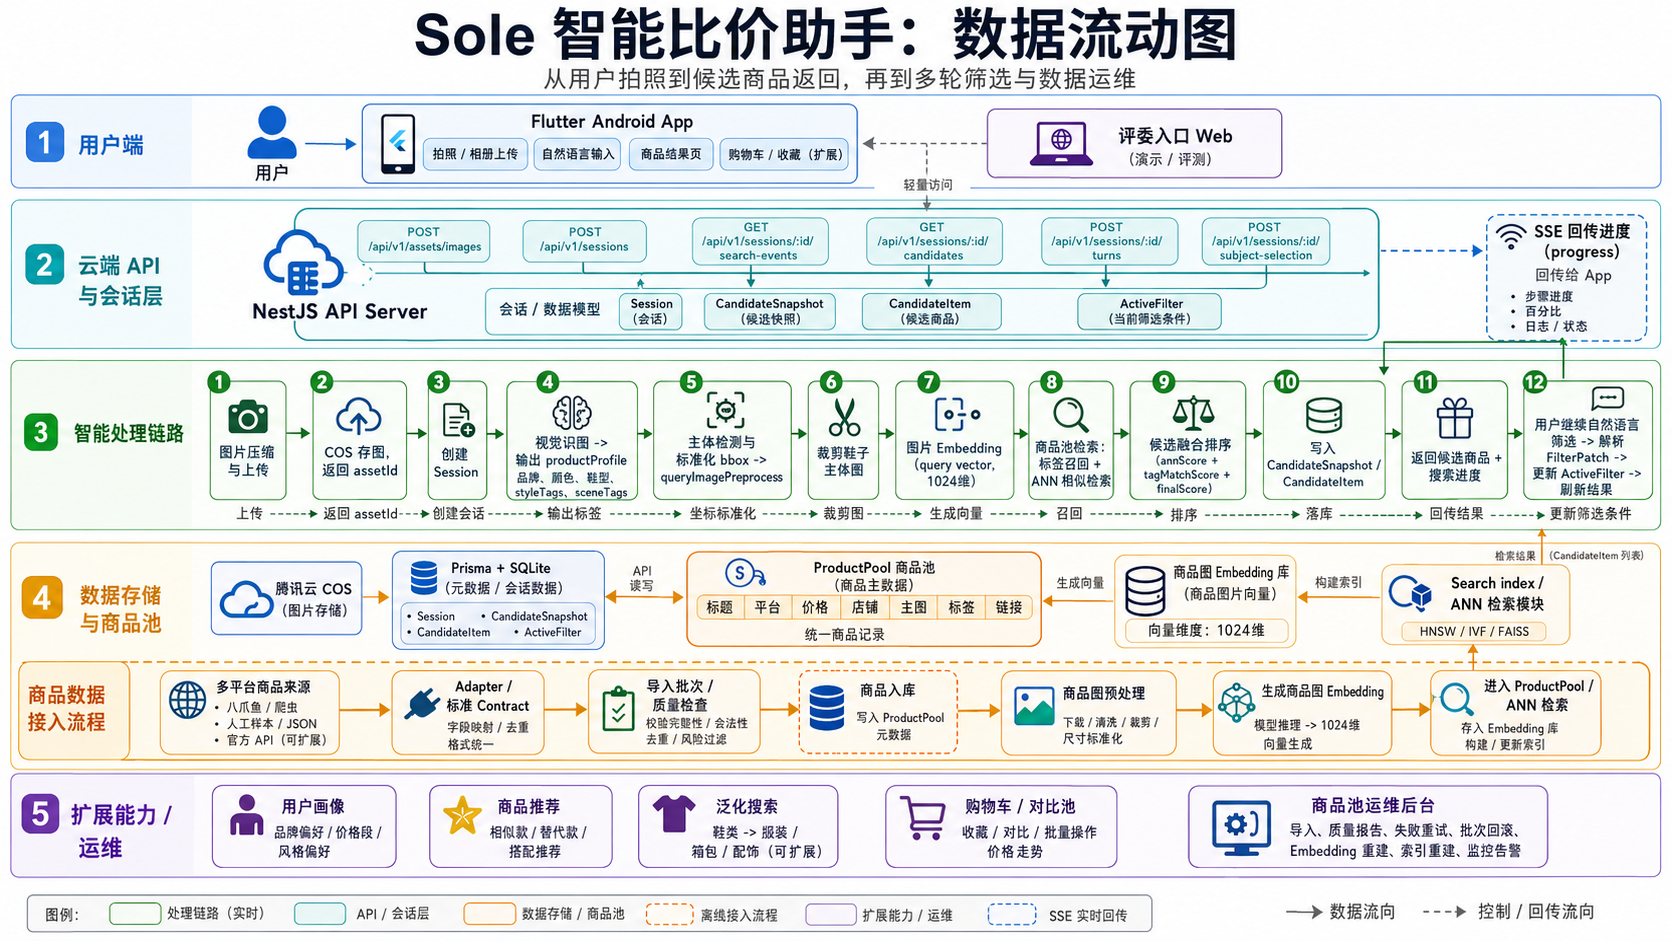
\includegraphics[width=0.82\textwidth]{architecture_overview.png}
  \vfill
  \begin{tabular}{ll}
    课程 & Human-Computer Interaction Final Project \\
    项目仓库 & \code{D:\textbackslash shopping-assistant} \\
    主要端形态 & Flutter Android App + NestJS API + Judge Entry Web \\
    团队成员 & 待补充：姓名、学号、分工 \\
    报告日期 & 2026 年 6 月 15 日 \\
  \end{tabular}
  \vfill
\end{titlepage}

\pagenumbering{Roman}
\tableofcontents
\newpage
\pagenumbering{arabic}

\section{摘要}

SoleAI 是一个面向全品类商品的智能比价助手。项目从用户在现实生活、社交媒体或电商页面中看到某件商品的场景出发，尝试把传统的“拍照识别、跨平台搜索、手动筛选、反复比较”压缩成一条连续的人机交互链路：用户上传或拍摄商品图，系统识别商品主体与关键标签，从真实商品池中召回候选结果，并允许用户继续用自然语言表达预算、平台、货源、风格等要求。本文中的手机截图主要以鞋类作为演示样例，但系统的数据结构、商品池、Adapter、检索链路和前端交互都按全品类购物助手组织。

从技术角度看，本项目采用 Flutter Android 客户端、NestJS 后端、Prisma + SQLite 数据层、腾讯云 COS 对象存储和 Zeabur 部署。核心检索链路采用“轻量标签召回 + 图片 ANN 召回 + 融合排序”的方案，这是在多次尝试后形成的折中：纯 ANN 返回快但解释性弱，完整识别后再检索更准但首屏等待长，混合 embedding 不利于用户修改标签后获得可解释反馈。最终方案把等待时间、搜索精确度和用户可控性放在同一条链路中平衡。项目还通过 Adapter / Provider / Port 把视觉模型、对话模型、商品数据源、对象存储、Embedding Provider 和 ANN 实现隔离在可替换边界后面，使全品类扩展不需要重写 App 主流程。

本报告以技术实现为主线，说明我们实际完成的程序结构、核心模块、关键技术取舍、系统优缺点和后续改进方向。报告同时加入手机界面截图、系统架构图和数据通路图，重点解释系统为什么这样设计，而不仅是罗列功能。

\noindent\textbf{English abstract for compatibility.} SoleAI is an all-category AI shopping assistant that supports visual product search, structured product understanding, multi-source candidate retrieval, natural-language refinement, and decision-oriented result presentation. The system combines a Flutter Android client, a NestJS API, a Prisma/SQLite product pool, object storage, model adapters, and a tag-plus-ANN retrieval pipeline to reduce users' search, filtering, and comparison workload.

\section{项目简介}

\subsection{问题背景}

传统电商搜索通常要求用户在多个平台之间切换：先拍照或输入关键词，再逐个平台搜索同款或相似商品，随后手动比较价格、店铺、库存、商品详情和购买链接。对于“我已经看到某件商品，只想尽快找到便宜可靠购买来源”的用户来说，困难不在于完全没有搜索入口，而在于搜索和判断过程被拆散在多个工具中：

\begin{itemize}
  \item 用户需要重复描述同一件商品。
  \item 每个平台的筛选条件、商品字段和结果排序都不一致。
  \item 用户追加条件时，传统筛选器往往要求重新设置多个按钮或重新输入关键词。
  \item 商品结果虽然很多，但缺少面向购买决策的解释和收敛。
\end{itemize}

SoleAI 的核心目标是减少这类重复操作，把用户输入方式收束为“图片 + 自然语言”，把系统输出方式收束为“可比较、可继续筛选、可进入详情判断的候选结果”。

\subsection{目标用户与使用场景}

项目面向全品类商品搜索与比价，特别适合已经看到明确目标商品、希望快速找到同款或近似款的用户。当前截图以鞋类商品作为演示样例，是因为鞋类具有明显外观、品牌、颜色和款式特征，便于展示视觉识别与标签修正能力；同一套链路也可用于数码、服饰、日用品等其他品类。典型场景如下：

\begin{enumerate}
  \item 用户在线下、短视频、社交平台或其他电商页面看到某件想买的商品。
  \item 用户打开 SoleAI，通过拍照或相册上传图片。
  \item 系统识别商品主体，生成品牌、颜色、品类、型号或款式等核心标签。
  \item 系统从商品池中召回候选商品，并展示平台、价格、图片、匹配信息和购买入口。
  \item 用户继续输入“500 元以内”“只看有货”“不要某个平台”等自然语言要求。
  \item 系统在同一会话中更新筛选条件和候选排序，帮助用户逐步完成购买判断。
\end{enumerate}

\subsection{HCI 设计目标}

项目的 HCI 目标不是单纯展示 AI 能力，而是降低用户在购物决策中的交互成本。表 \ref{tab:hci-goals} 总结了主要设计目标。

\begin{table}[H]
\centering
\caption{HCI 设计目标与对应实现}
\label{tab:hci-goals}
\begin{tabularx}{\textwidth}{p{3.2cm}Y Y}
\toprule
目标 & 用户侧问题 & 项目中的实现方式 \\
\midrule
减少输入成本 & 用户不想反复输入商品名、品牌、颜色和筛选条件 & 以拍照或相册上传作为入口，系统自动识别商品主体和核心标签 \\
减少筛选成本 & 用户追加需求时不想逐个调整筛选器 & 支持多轮自然语言收敛，后端把语言要求合并为结构化筛选状态 \\
减少比较成本 & 用户需要在多个平台和多个商品间做判断 & 候选卡片统一展示价格、平台、货源、匹配摘要和推荐理由 \\
减少中断成本 & 模型或外部数据失败会破坏体验 & 使用缓存、快照和降级路径，尽量保持会话可恢复 \\
增强可控性 & AI 识别可能出错，用户需要纠正 & 前端展示可编辑识别标签，用户保存后触发重新检索 \\
\bottomrule
\end{tabularx}
\end{table}

\subsection{核心用户旅程}

图 \ref{fig:user-journey} 展示从用户输入到购买判断的主路径。该路径将图片理解、检索、筛选、建议和详情组织为一个连续体验。

\begin{figure}[H]
\centering
\resizebox{\textwidth}{!}{
\begin{tikzpicture}[
  node distance=1.25cm,
  journey/.style={rectangle, rounded corners=2pt, draw=soleBlue, fill=lightBlue, minimum width=2.5cm, minimum height=0.95cm, align=center},
  support/.style={rectangle, rounded corners=2pt, draw=soleGreen, fill=lightGreen, minimum width=2.55cm, minimum height=0.95cm, align=center},
  arrow/.style={-{Stealth[length=2.4mm]}, thick, draw=soleGray}
]
\node[journey] (input) {拍照/上传\\商品图片};
\node[journey, right=of input] (bbox) {主体框选\\与确认};
\node[journey, right=of bbox] (profile) {商品画像\\核心标签};
\node[journey, right=of profile] (retrieve) {标签 + ANN\\候选召回};
\node[journey, right=of retrieve] (list) {统一候选\\结果列表};
\node[support, below=of list] (refine) {自然语言\\多轮筛选};
\node[support, left=of refine] (decision) {建议卡片\\决策辅助};
\node[support, left=of decision] (detail) {商品详情\\购买入口};
\draw[arrow] (input) -- (bbox);
\draw[arrow] (bbox) -- (profile);
\draw[arrow] (profile) -- (retrieve);
\draw[arrow] (retrieve) -- (list);
\draw[arrow] (list) -- (refine);
\draw[arrow] (refine) -- (decision);
\draw[arrow] (decision) -- (detail);
\draw[arrow] (refine.north) to[bend left=18] node[above, font=\small] {刷新筛选条件与排序} (list.south);
\end{tikzpicture}
}
\caption{面向用户购物决策的核心旅程}
\label{fig:user-journey}
\end{figure}

\section{程序结构与模块}

\subsection{总体架构}

项目采用移动端、API 服务、商品池、模型适配器和对象存储协作的结构。客户端保持轻量，负责图片采集、会话展示和交互状态；后端负责会话编排、图片处理、模型调用、商品检索、候选快照和多轮筛选。

\begin{figure}[H]
\centering
\resizebox{\textwidth}{!}{
\begin{tikzpicture}[
  layer/.style={rectangle, rounded corners=3pt, draw=black!45, fill=lightGray, minimum width=4.1cm, minimum height=1cm, align=center},
  api/.style={rectangle, rounded corners=3pt, draw=soleBlue, fill=lightBlue, minimum width=3.7cm, minimum height=0.9cm, align=center},
  data/.style={rectangle, rounded corners=3pt, draw=soleGreen, fill=lightGreen, minimum width=3.7cm, minimum height=0.9cm, align=center},
  ext/.style={rectangle, rounded corners=3pt, draw=soleOrange, fill=lightOrange, minimum width=3.7cm, minimum height=0.9cm, align=center},
  arrow/.style={-{Stealth[length=2.2mm]}, thick, draw=soleGray}
]
\node[layer] (client) {Flutter Android 客户端\\拍照、相册、结果页、详情页};
\node[api, right=1.1cm of client] (api) {NestJS API\\会话、候选、画像、推荐};
\node[data, right=1.1cm of api] (db) {Prisma + SQLite\\会话、快照、商品池};
\node[ext, below=0.9cm of api] (models) {Model Adapter\\视觉识别、对话解析、建议生成};
\node[ext, below=0.9cm of db] (storage) {对象存储 + Embedding\\COS、图片向量、ANN Port};
\node[data, above=0.9cm of db] (web) {Judge Entry Web\\APK 入口、说明、运维页};
\draw[arrow] (client) -- node[above, font=\small] {HTTP / JSON / multipart} (api);
\draw[arrow] (api) -- node[above, font=\small] {Repository / View Adapter} (db);
\draw[arrow] (api) -- (models);
\draw[arrow] (api) -- (storage);
\draw[arrow] (web) -- (api);
\draw[arrow] (storage) -- (db);
\end{tikzpicture}
}
\caption{系统总体架构}
\label{fig:architecture}
\end{figure}

\subsection{目录结构}

当前仓库的主要目录与职责如下：

\begin{table}[H]
\centering
\caption{项目目录与职责}
\begin{tabularx}{\textwidth}{p{4.2cm}Y}
\toprule
目录 & 职责 \\
\midrule
\code{apps/mobile-flutter} & Flutter Android 客户端，承载拍照、相册、主体选择、候选结果、自然语言输入、详情页、用户画像和购物车交互。 \\
\code{apps/judge-entry-web} & 评委入口 Web 页，承载项目介绍、APK 下载说明和商品池可视化运维入口。 \\
\code{services/api-server} & NestJS API 服务，承载会话、图片上传、商品画像、候选检索、多轮筛选、用户记忆、TrendOutfit 推荐等业务逻辑。 \\
\code{docs} & 项目定义、技术方案、接口契约、测试验收、部署说明和课程提交材料。 \\
\code{samples} / \code{scripts} & 商品池样例、导入脚本、数据清洗脚本和 smoke 验证脚本。 \\
\code{infra/zeabur} & Zeabur 部署说明和相关配置。 \\
\bottomrule
\end{tabularx}
\end{table}

\subsection{核心后端模块}

后端不是把所有逻辑写在控制器中，而是以模块和 Adapter 组织。这样做的原因是本项目涉及图片、模型、商品数据、向量检索、会话状态和前端视图，如果全部混在一个搜索函数里，后续扩品类或替换数据源时会变得不可维护。我们实际完成的后端能力可以概括为“会话编排 + 商品池资产化 + 可解释检索 + 多轮收敛”。

\begin{itemize}
  \item \textbf{Assets 模块}：接收用户上传图，记录图片元数据，保存对象存储引用。它解决的是“图片本体不要进入数据库”的问题，数据库只保存 objectKey、URL、尺寸、来源和变体类型。
  \item \textbf{Sessions 模块}：创建查询会话，组织商品理解、图片裁剪、候选召回和候选快照写入。它是主链路编排层，避免前端直接调用多个模型和数据源。
  \item \textbf{ProductPool 模块}：维护真实商品池，支持多平台、多品类商品导入、批次管理、图片 embedding、可检索状态和运维查询。商品池不是 mock 列表，而是项目的核心数据资产。
  \item \textbf{Search / ANN 模块}：将标签召回和图片向量召回融合，输出标准候选。它承担等待时间和搜索准确度之间的平衡。
  \item \textbf{Turns / Conversation 模块}：解析用户自然语言追加要求，更新筛选状态并刷新候选结果。用户说“便宜一点”“只看某平台”“排除某来源”时，不会重新开始一次无上下文搜索。
  \item \textbf{Suggestions 模块}：基于当前候选和筛选状态生成建议卡与决策辅助信息，把候选结果转成更接近购买判断的表达。
  \item \textbf{User Memory 模块}：支持用户画像块、待确认记忆、尺码/预算/平台偏好等长期偏好能力。长期记忆采用用户确认后写入的策略，避免 AI 自动保存错误偏好。
  \item \textbf{TrendOutfit 模块}：从会话购物车或候选商品出发，生成搭配推荐。该模块保持独立接口，不混入主搜索链路，避免影响基础图片搜索稳定性。
  \item \textbf{Cache 模块}：提供进程内轻缓存，用于 ANN、识别、搜索和推荐结果复用。缓存只是加速层，正式会话状态仍以 SQLite 快照为准。
\end{itemize}

\subsection{可插拔工程设计}

项目的重要工程特点是把外部依赖放在可替换边界后面。核心服务消费稳定 contract，而不是直接依赖某个模型、平台字段或对象存储 SDK。图 \ref{fig:adapter} 展示了这种分层方式。

\begin{figure}[H]
\centering
\resizebox{0.96\textwidth}{!}{
\begin{tikzpicture}[
  node distance=0.8cm,
  block/.style={rectangle, rounded corners=2pt, draw=soleGray, fill=lightGray, minimum width=3.1cm, minimum height=0.75cm, align=center},
  core/.style={rectangle, rounded corners=2pt, draw=soleBlue, fill=lightBlue, minimum width=3.1cm, minimum height=0.75cm, align=center},
  arrow/.style={-{Stealth[length=2.2mm]}, thick, draw=soleGray}
]
\node[block] (external) {外部能力\\模型、平台、存储、向量库};
\node[block, right=of external] (adapter) {Adapter / Provider / Port};
\node[core, right=of adapter] (contract) {标准 Contract\\Product / Session / Candidate};
\node[core, right=of contract] (service) {Core Service\\会话编排与业务规则};
\node[block, right=of service] (view) {View Adapter\\API 响应};
\draw[arrow] (external) -- (adapter);
\draw[arrow] (adapter) -- (contract);
\draw[arrow] (contract) -- (service);
\draw[arrow] (service) -- (view);
\end{tikzpicture}
}
\caption{外部能力到稳定业务对象的可插拔边界}
\label{fig:adapter}
\end{figure}

这一设计直接服务于 HCI 体验：用户不需要理解模型供应商、商品平台、向量检索和对象存储差异；系统用统一界面承接复杂后端能力，并且在能力替换时尽量保持前端交互不变。

在实现过程中，这种可插拔结构并不是为了“架构好看”而设计的。项目一开始容易走向两种简单但不可持续的路线：一种是直接把某个采集工具返回的字段写进搜索流程，另一种是把模型自由文本直接传给前端展示。前者会导致一换平台就要改业务逻辑，后者会导致结果不可校验、不可回放、不可排序。最终实现中，我们把外部数据先收敛到标准商品契约，把模型输出先收敛到标准画像和筛选 patch，再让核心服务处理稳定对象。这也是全品类能力的基础：新增品类时主要增加品类字段、Prompt、标签映射和展示字段，而不是重写上传、会话、候选、分页和推荐流程。

具体来说，商品数据源可替换意味着淘宝、京东、苏宁、唯品会、闲鱼或其他来源的数据都先进入 ProductImportAdapter；模型可替换意味着视觉识别、对话解析和建议文案都通过 ModelAdapter；检索可替换意味着当前应用内 ANN 将来可以替换成 sqlite-vec、pgvector 或专门向量库；对象存储可替换意味着腾讯云 COS 将来可以替换成 OSS、S3 或本地存储。对用户来说，这些替换不应该改变“拍照 - 看结果 - 继续筛选”的主体验。

\section{关键交互流程与界面}

\subsection{移动端主流程}

图 \ref{fig:mobile-flow} 展示了移动端从首页、主体框选、等待搜索、编辑识别标签到结果列表的流程。首页突出输入入口，主体选择页让用户纠正识别范围，结果页则把候选、筛选条件和后续对话统一放在同一个上下文中。

这里的交互不是简单把后端能力逐页展示出来，而是按照用户完成一次购物决策的顺序组织。首页不要求用户先填写复杂筛选器，而是让用户用拍照、相册或一句自然语言开始；主体框选页把“模型可能看错主体”这个风险提前暴露给用户，让用户有机会纠正；搜索等待页不只显示加载动画，而是展示当前用于搜索的条件和系统进度；标签编辑页只暴露核心标签，避免把完整模型 JSON 交给用户；结果页把候选列表、继续追问、建议卡片和购物车入口放在同一个会话环境中，减少用户在页面之间来回切换。

\begin{figure}[H]
\centering
\begin{subfigure}{0.19\textwidth}
  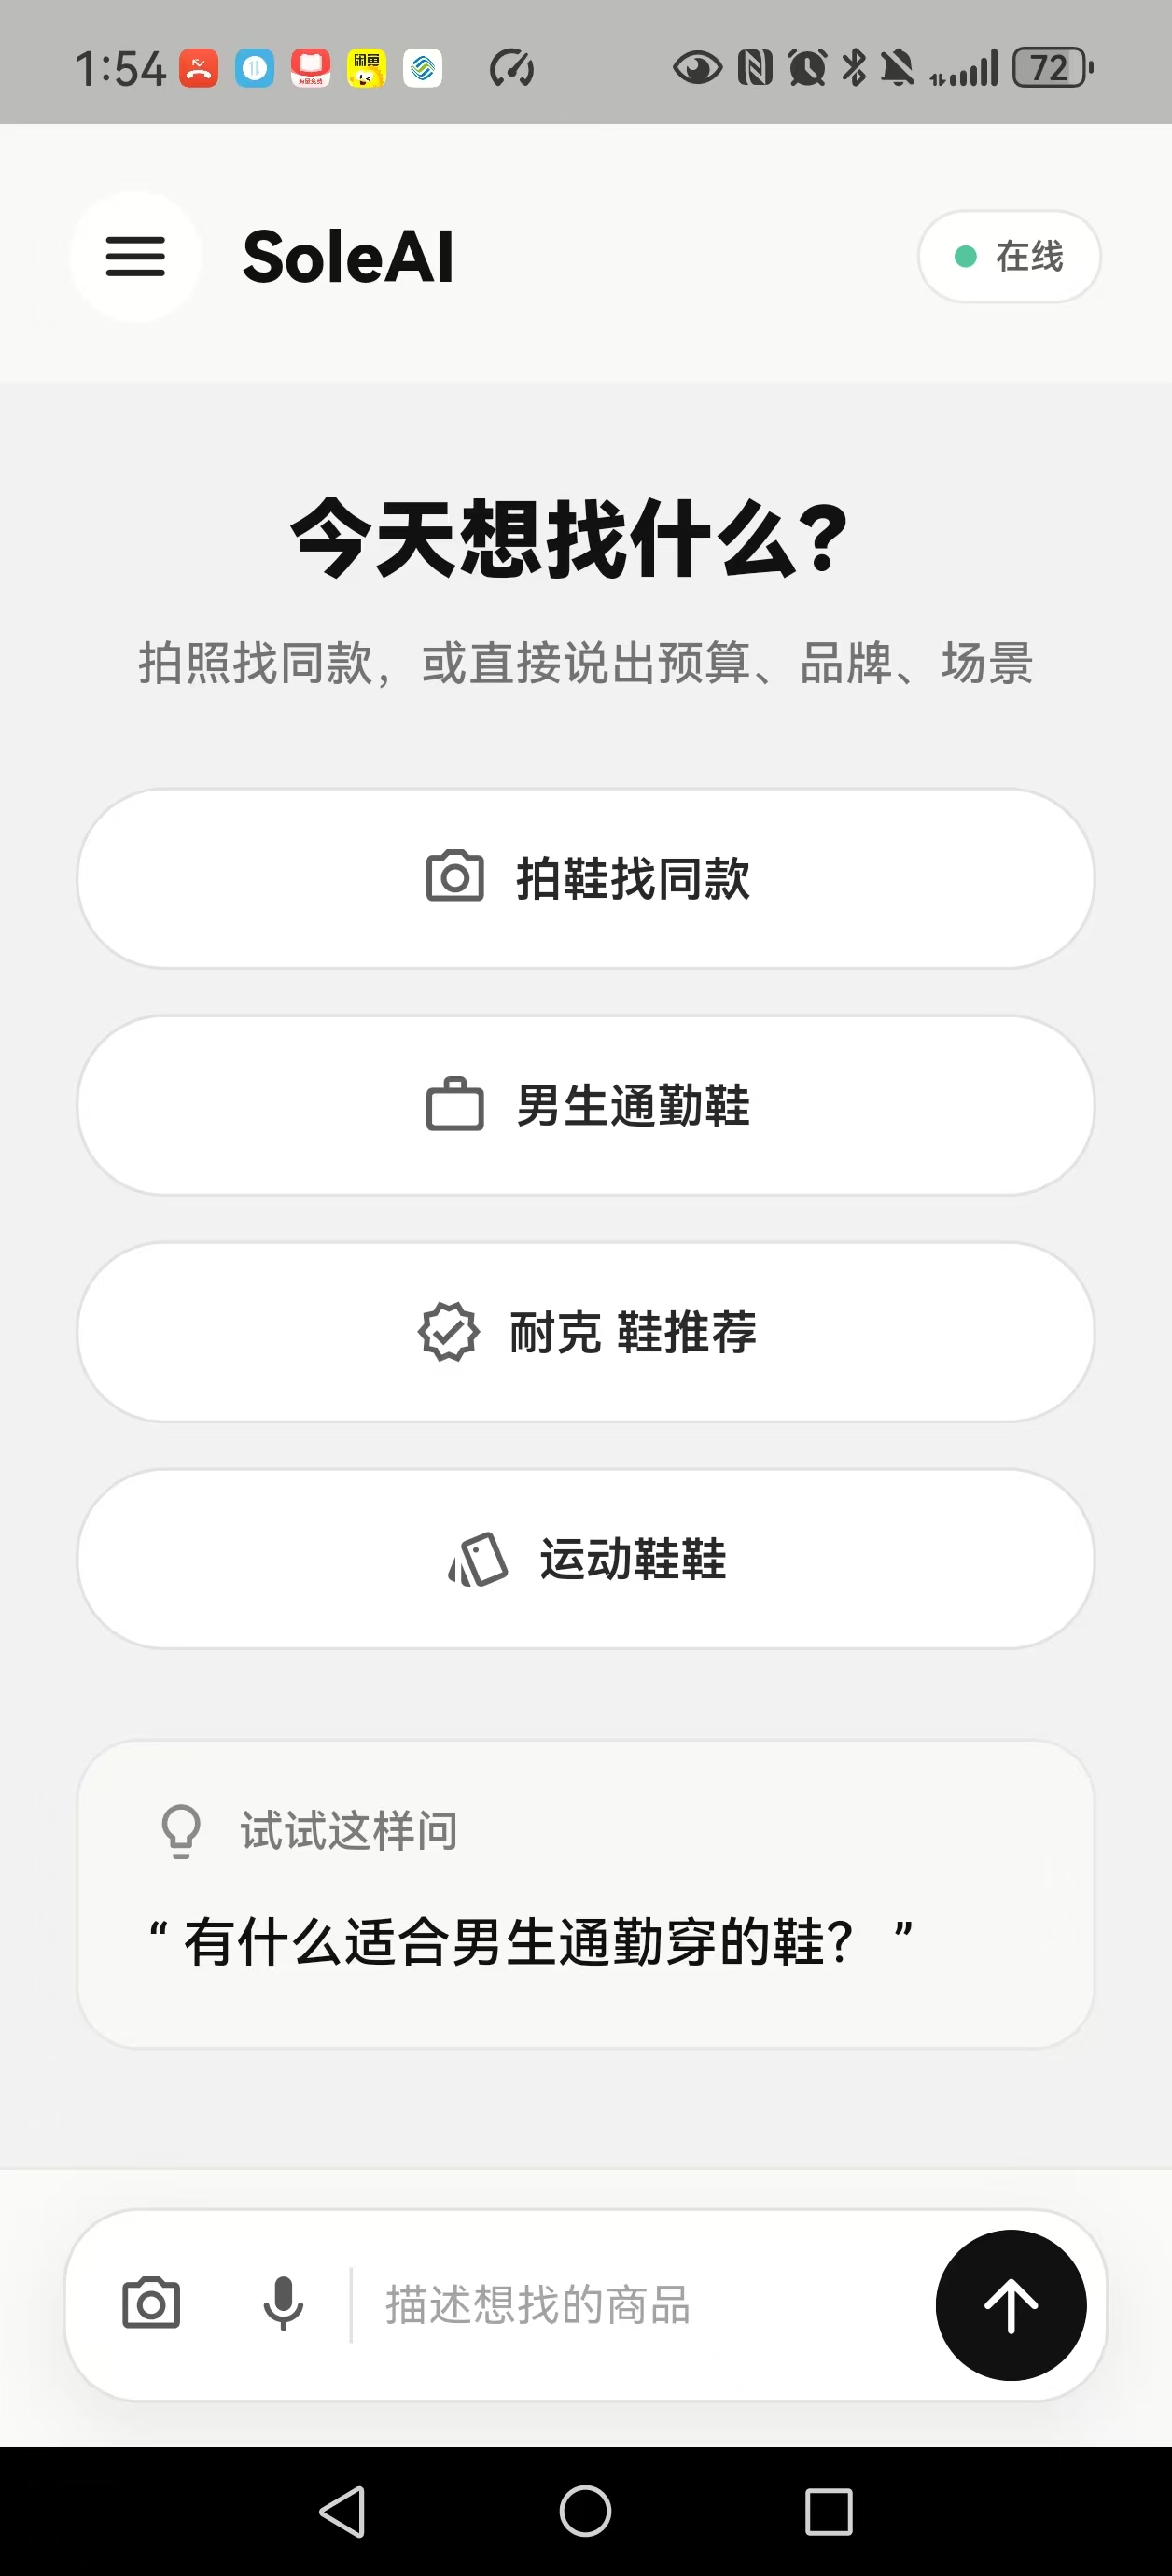
\includegraphics[width=\linewidth]{ui_home.jpg}
  \caption{首页}
\end{subfigure}
\hfill
\begin{subfigure}{0.19\textwidth}
  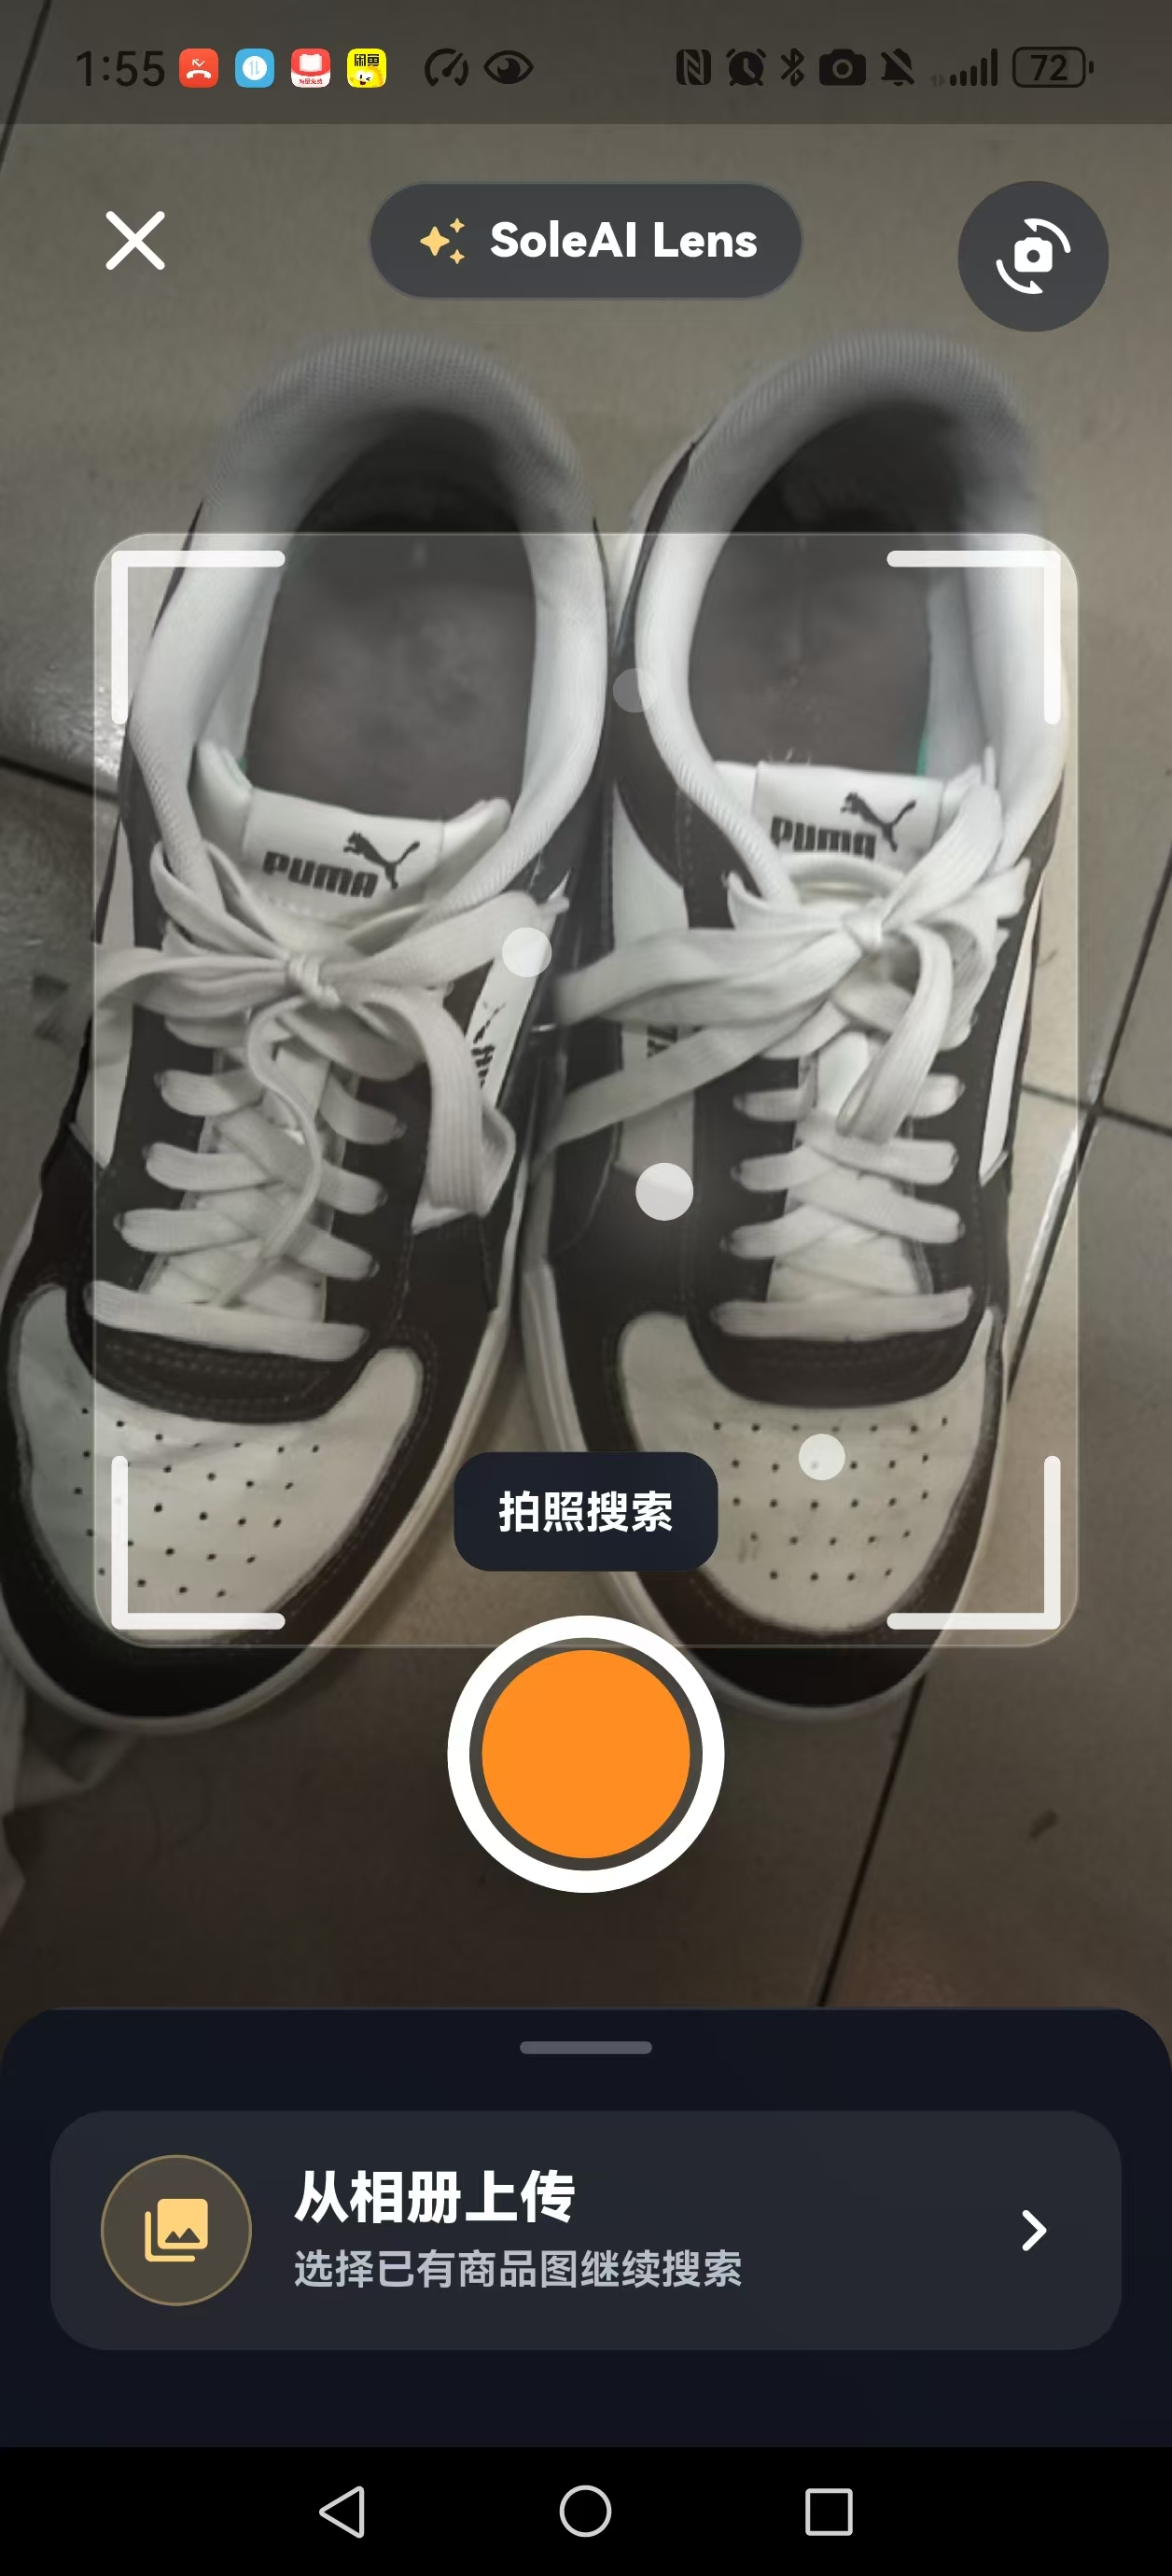
\includegraphics[width=\linewidth]{ui_subject_selection.jpg}
  \caption{主体框选}
\end{subfigure}
\hfill
\begin{subfigure}{0.19\textwidth}
  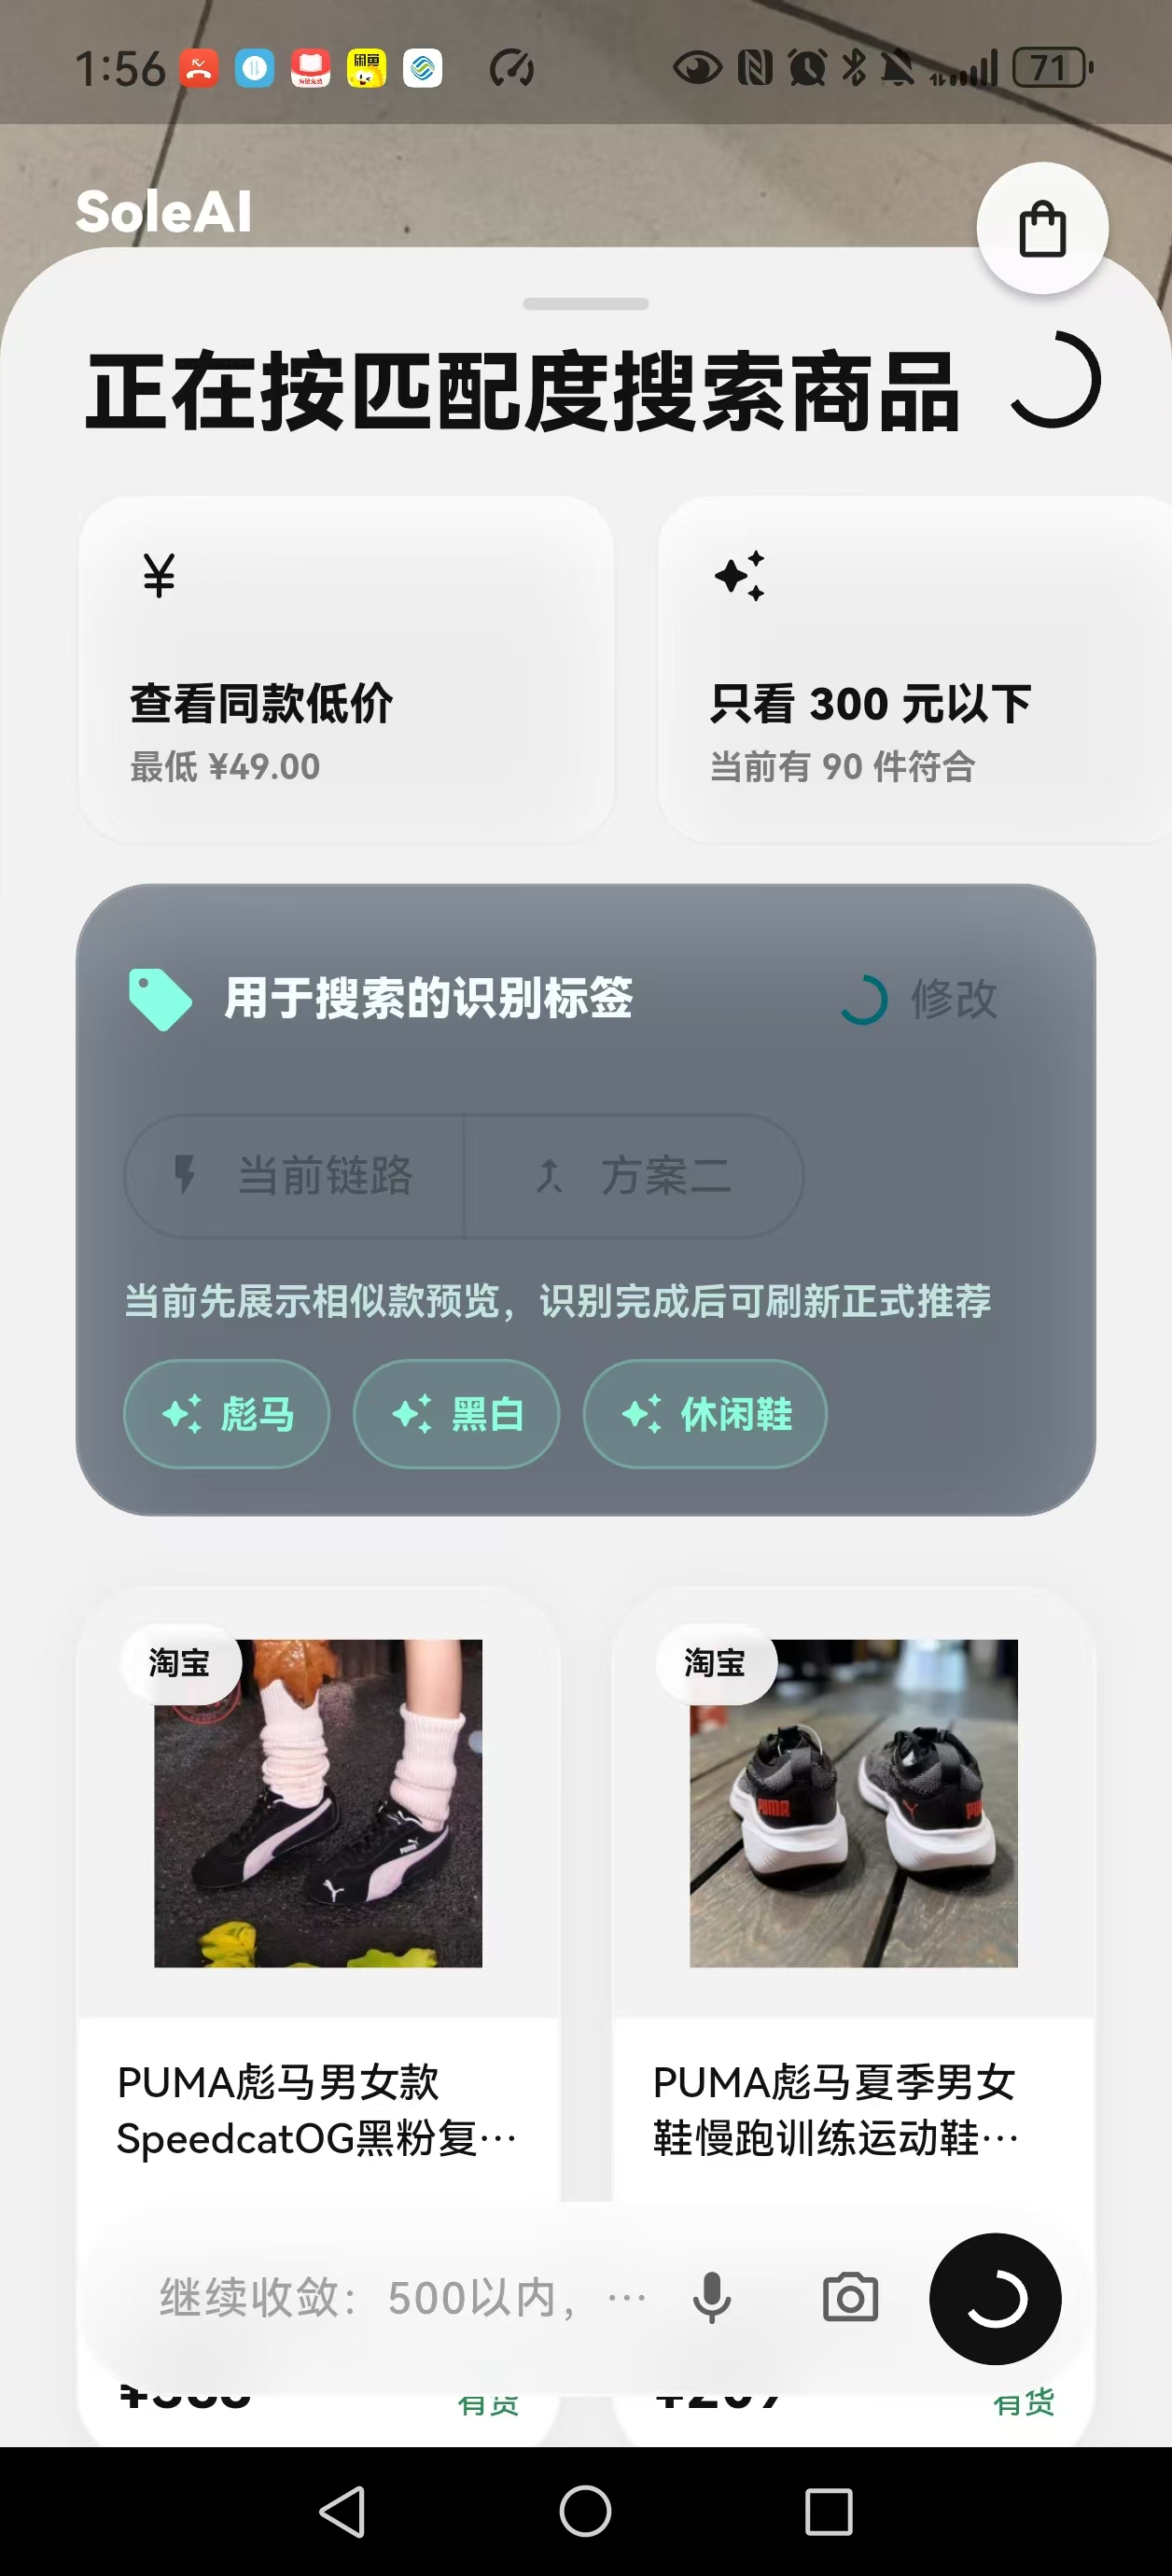
\includegraphics[width=\linewidth]{ui_loading_results.jpg}
  \caption{搜索中}
\end{subfigure}
\hfill
\begin{subfigure}{0.19\textwidth}
  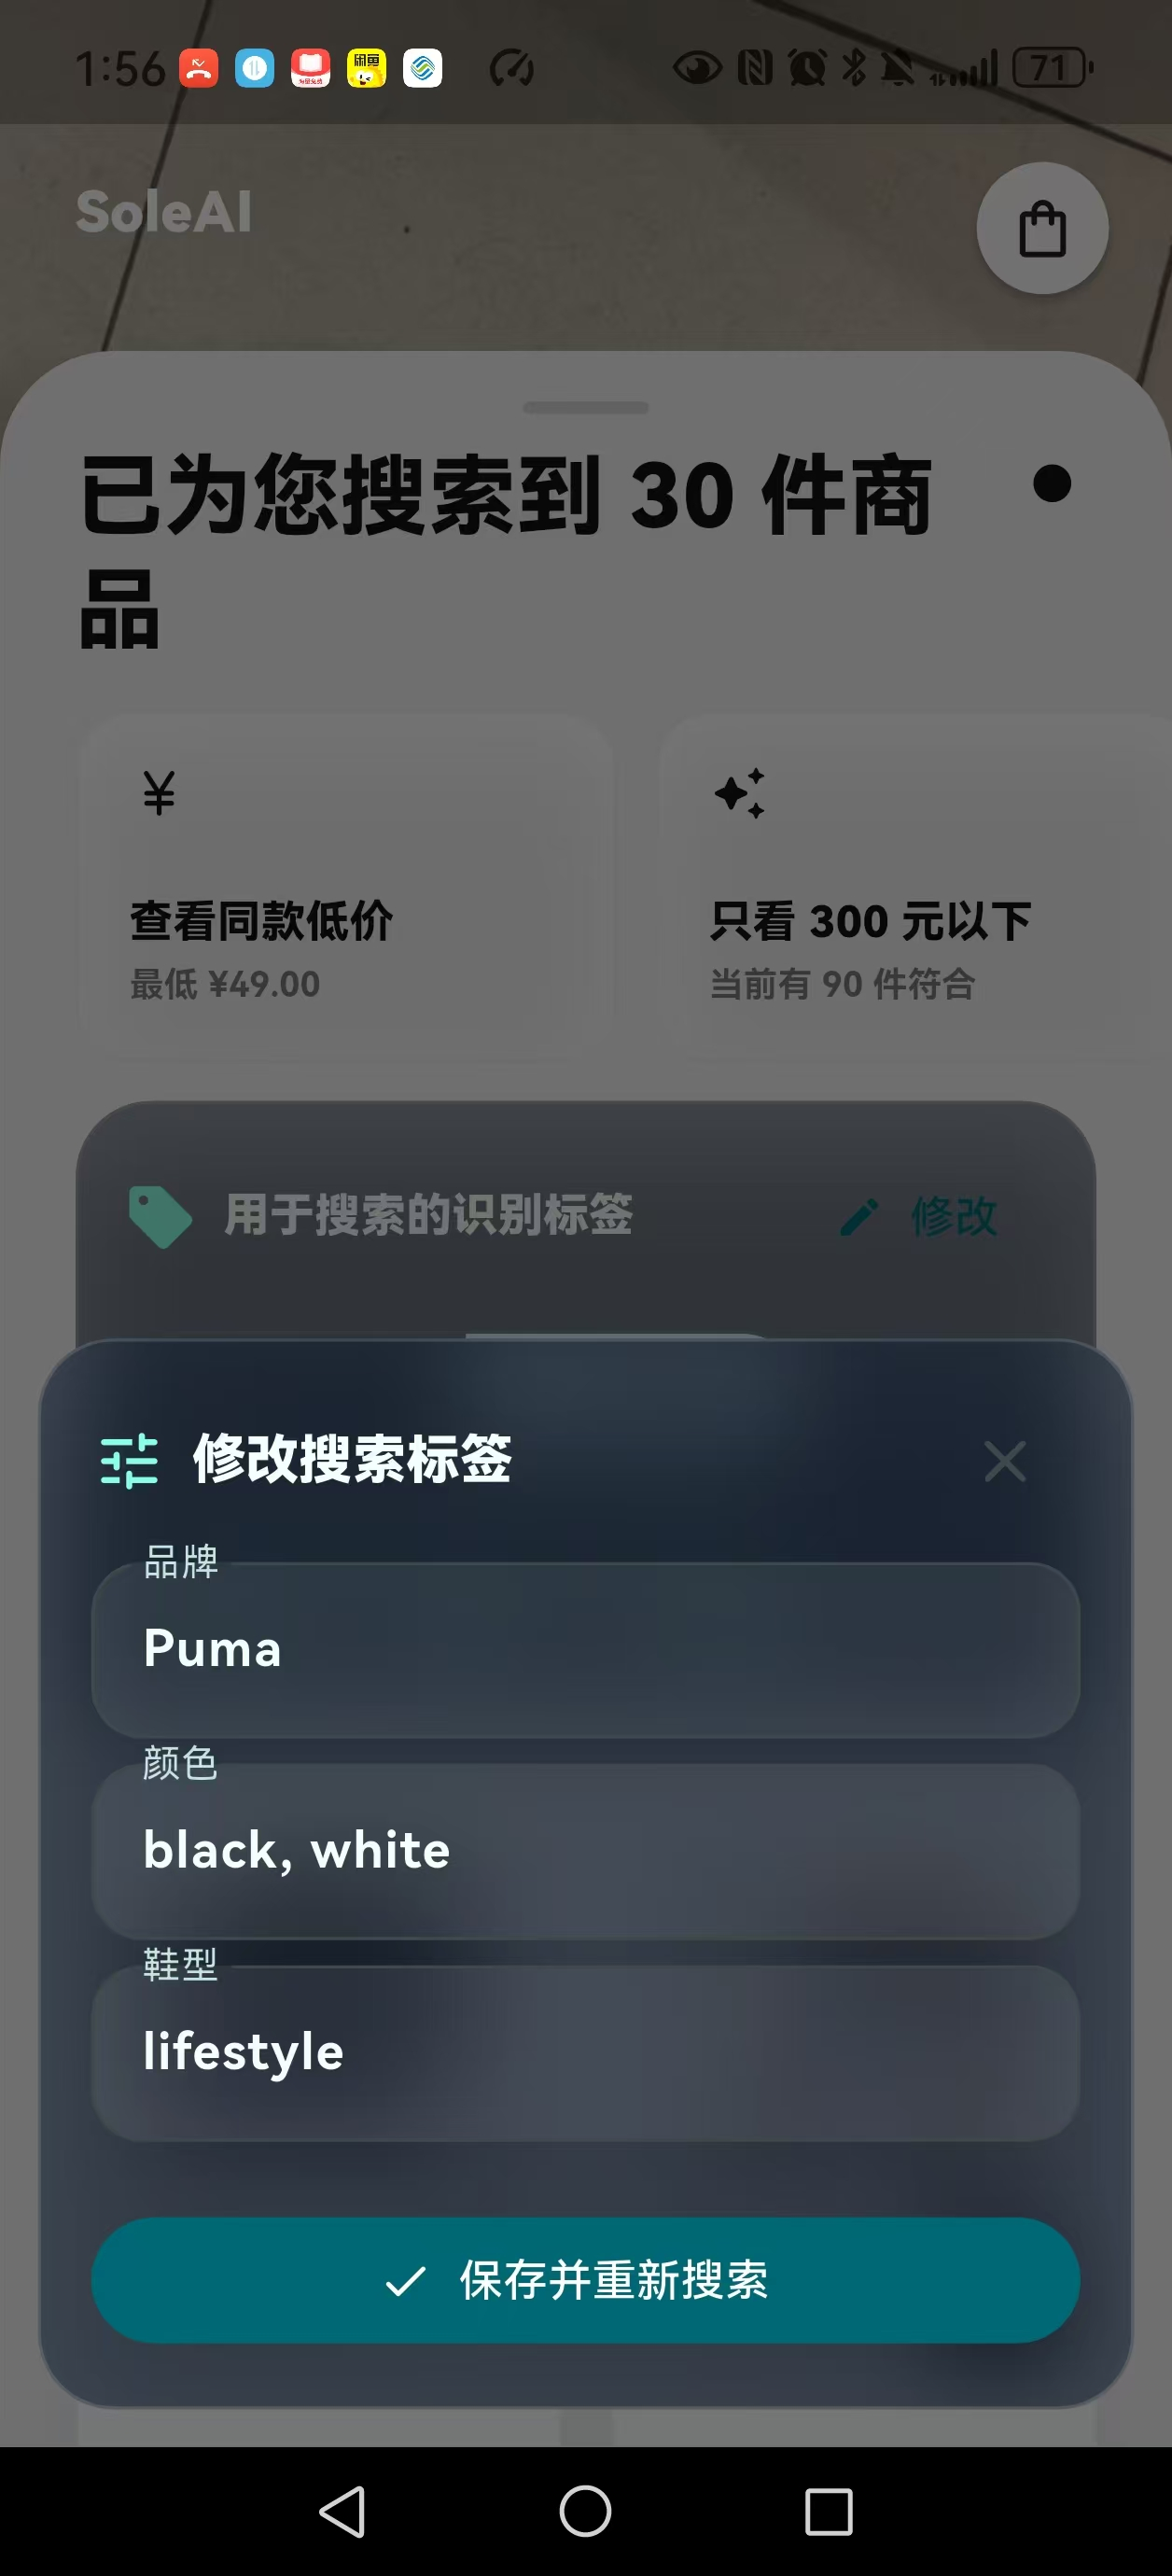
\includegraphics[width=\linewidth]{ui_editable_profile.jpg}
  \caption{标签编辑}
\end{subfigure}
\hfill
\begin{subfigure}{0.19\textwidth}
  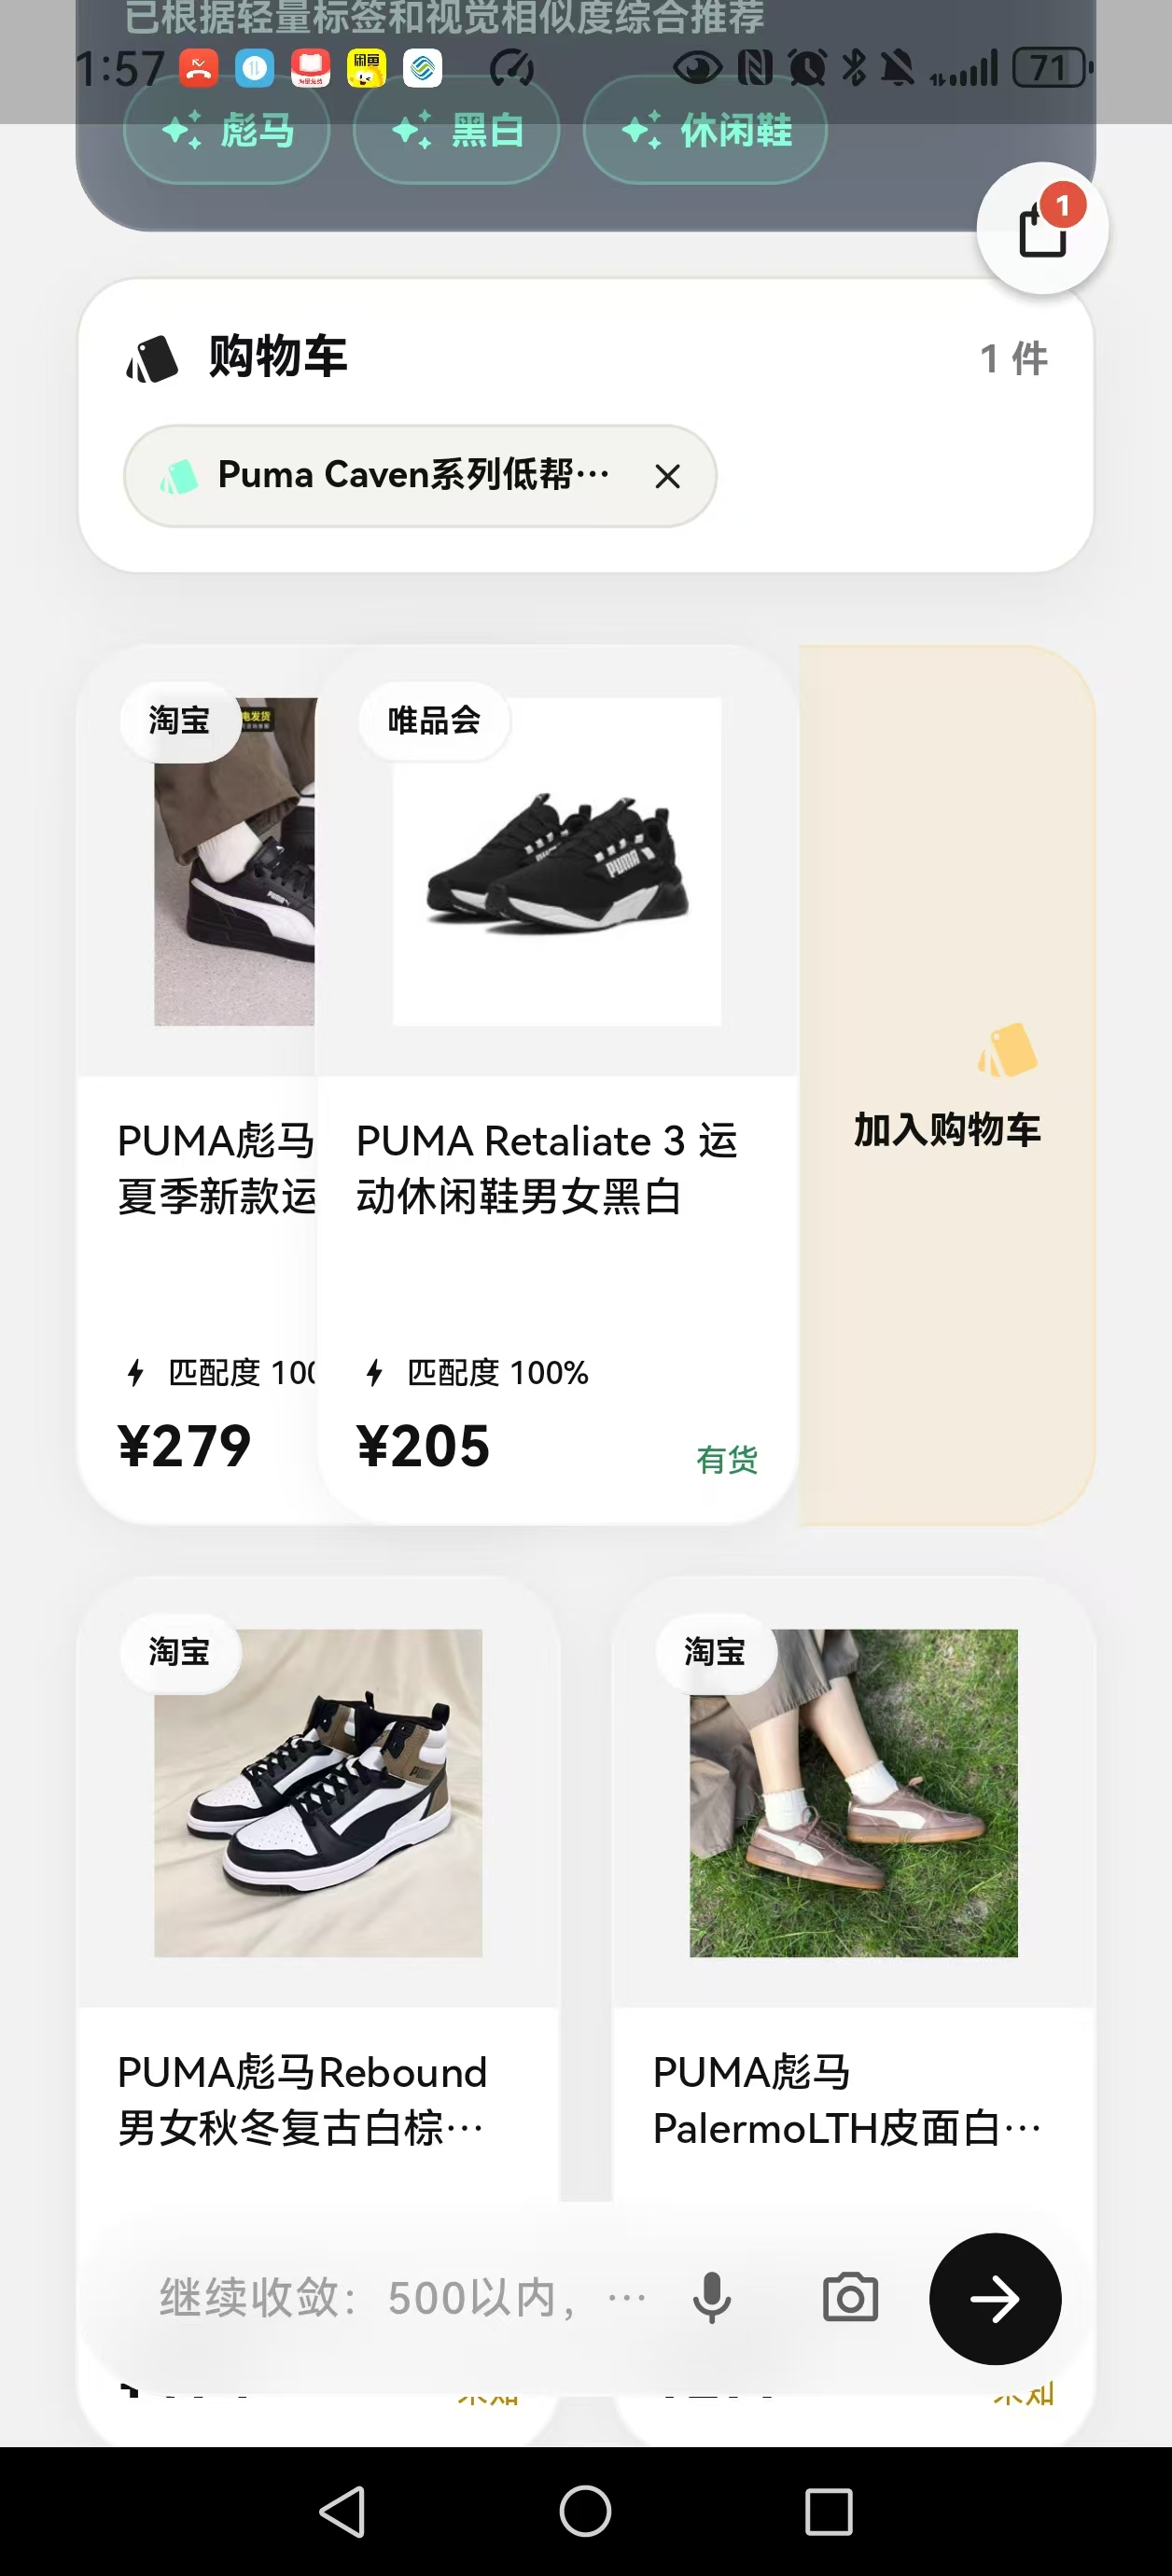
\includegraphics[width=\linewidth]{ui_result_grid.jpg}
  \caption{结果列表}
\end{subfigure}
\caption{Flutter 移动端主流程截图}
\label{fig:mobile-flow}
\end{figure}

\subsection{多轮筛选与决策辅助}

用户进入结果页后，可以继续输入自然语言要求，例如“我想要 500 元以下的平台产品”“只看有货”“不要某个平台”等。系统会把这些表达合并到当前会话的筛选状态，并基于候选快照刷新展示结果。图 \ref{fig:refine-ui} 展示了自然语言筛选、商品详情和外部商品页之间的关系。

我们没有把自然语言输入做成一个独立聊天机器人，因为那样容易让购物任务发散。当前设计中，自然语言的作用是修改当前会话的筛选状态，例如预算、平台偏好、货源状态、排除条件或排序倾向。后端会把这些要求合并进 activeFilter，并基于当前 CandidateSnapshot 过滤、重排或补充检索。这样用户说出的每一句话都服务于结果收敛，而不是产生一段脱离商品事实的聊天回复。

\begin{figure}[H]
\centering
\begin{subfigure}{0.23\textwidth}
  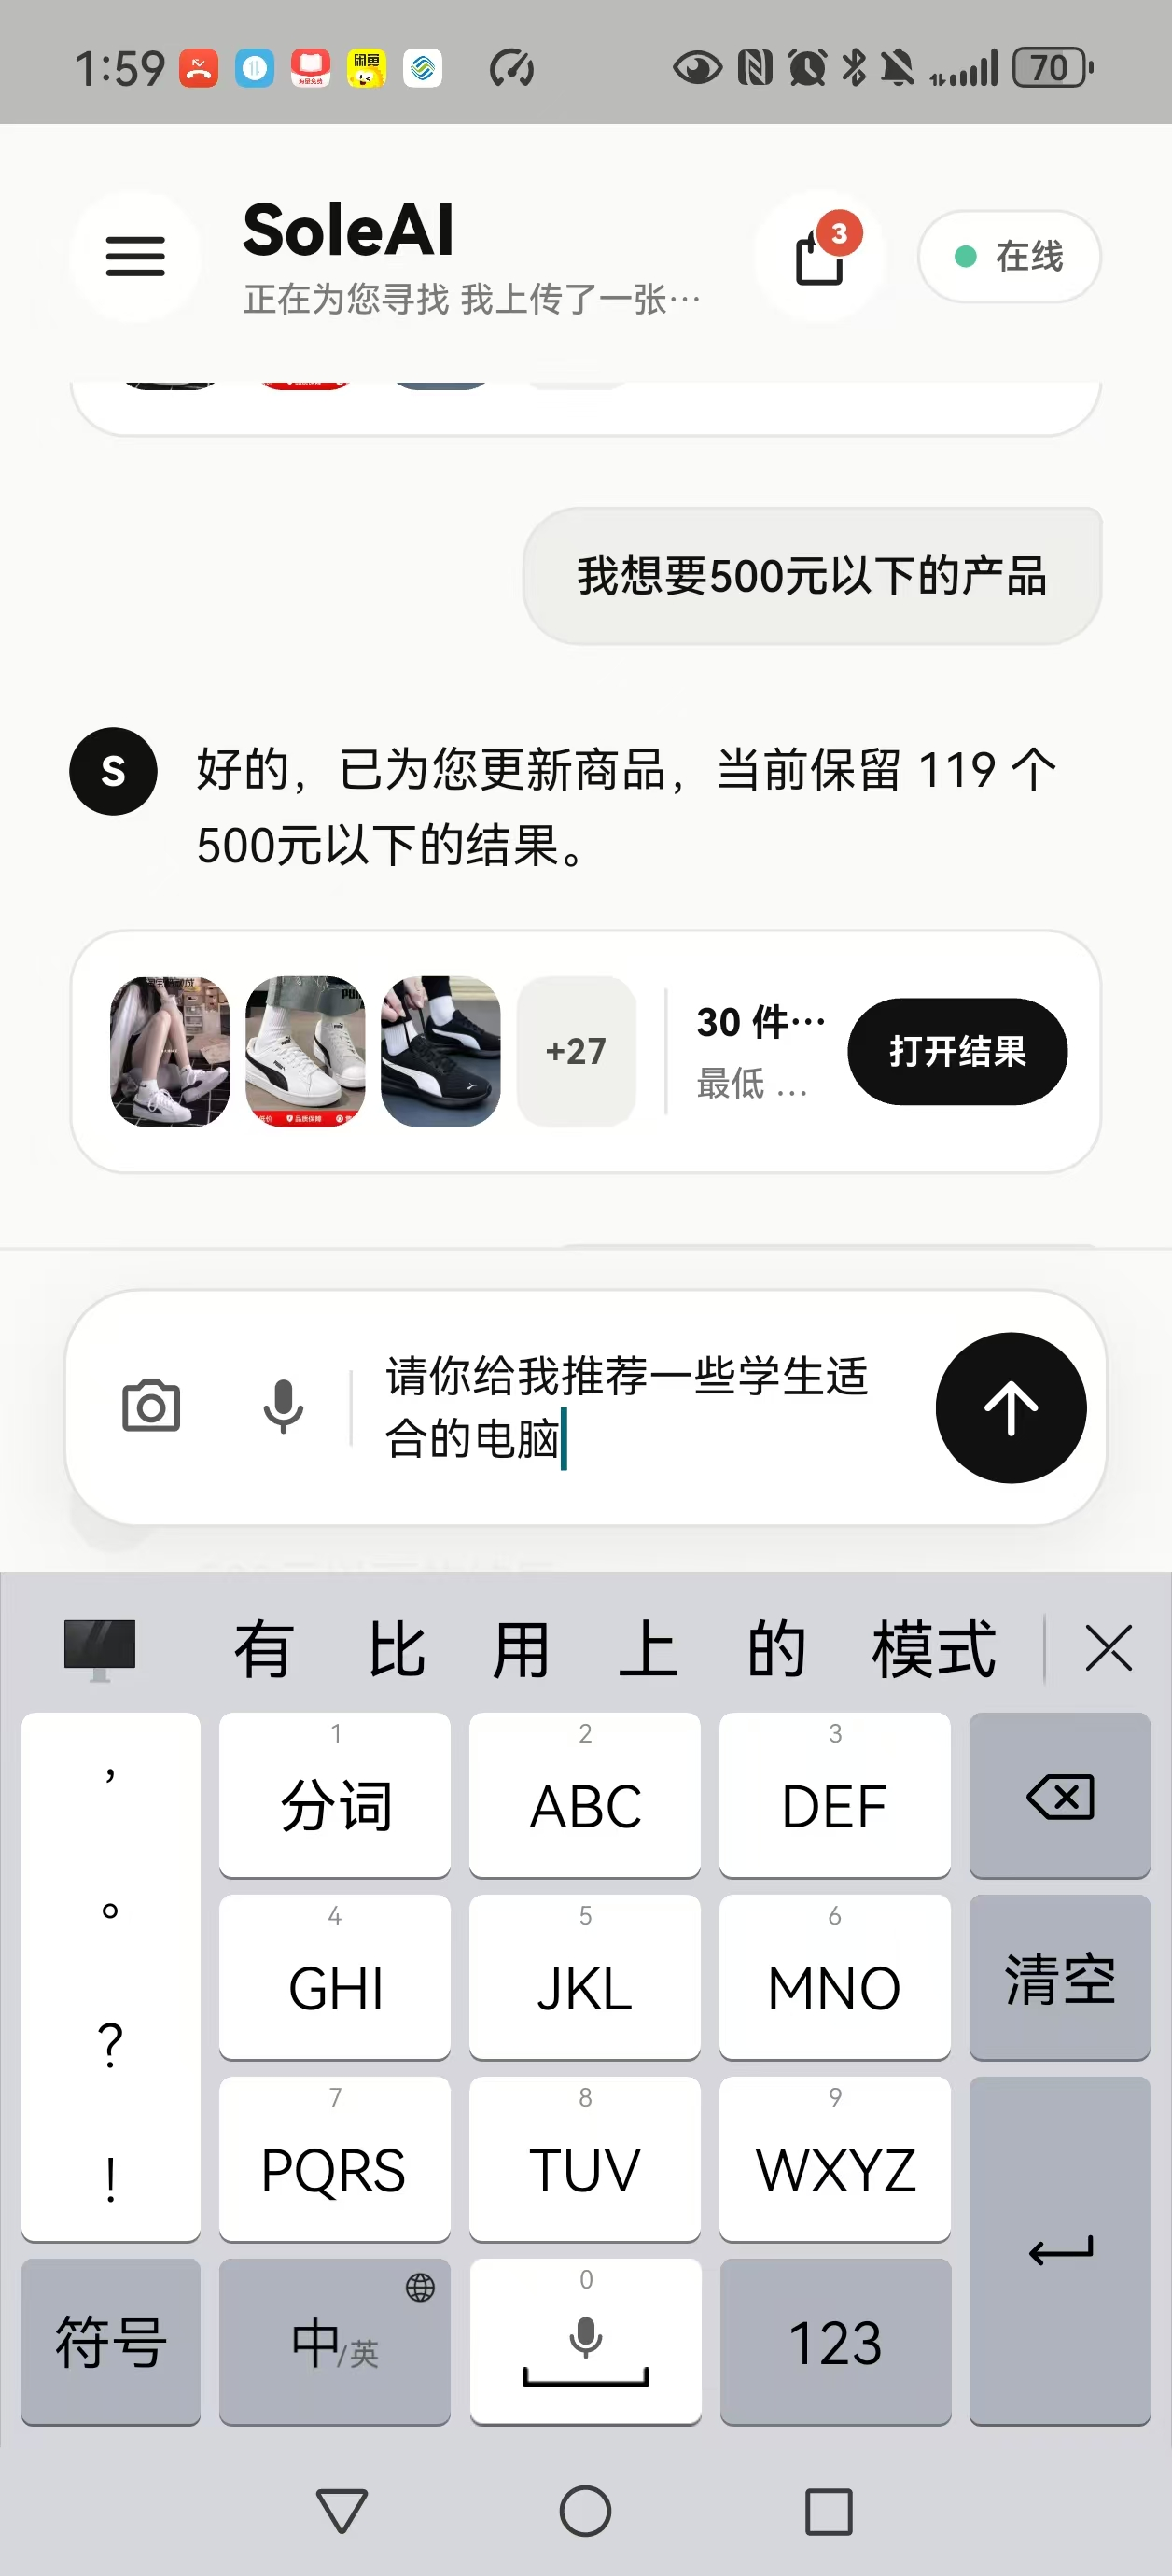
\includegraphics[width=\linewidth]{ui_nl_refinement.jpg}
  \caption{自然语言追问}
\end{subfigure}
\hfill
\begin{subfigure}{0.23\textwidth}
  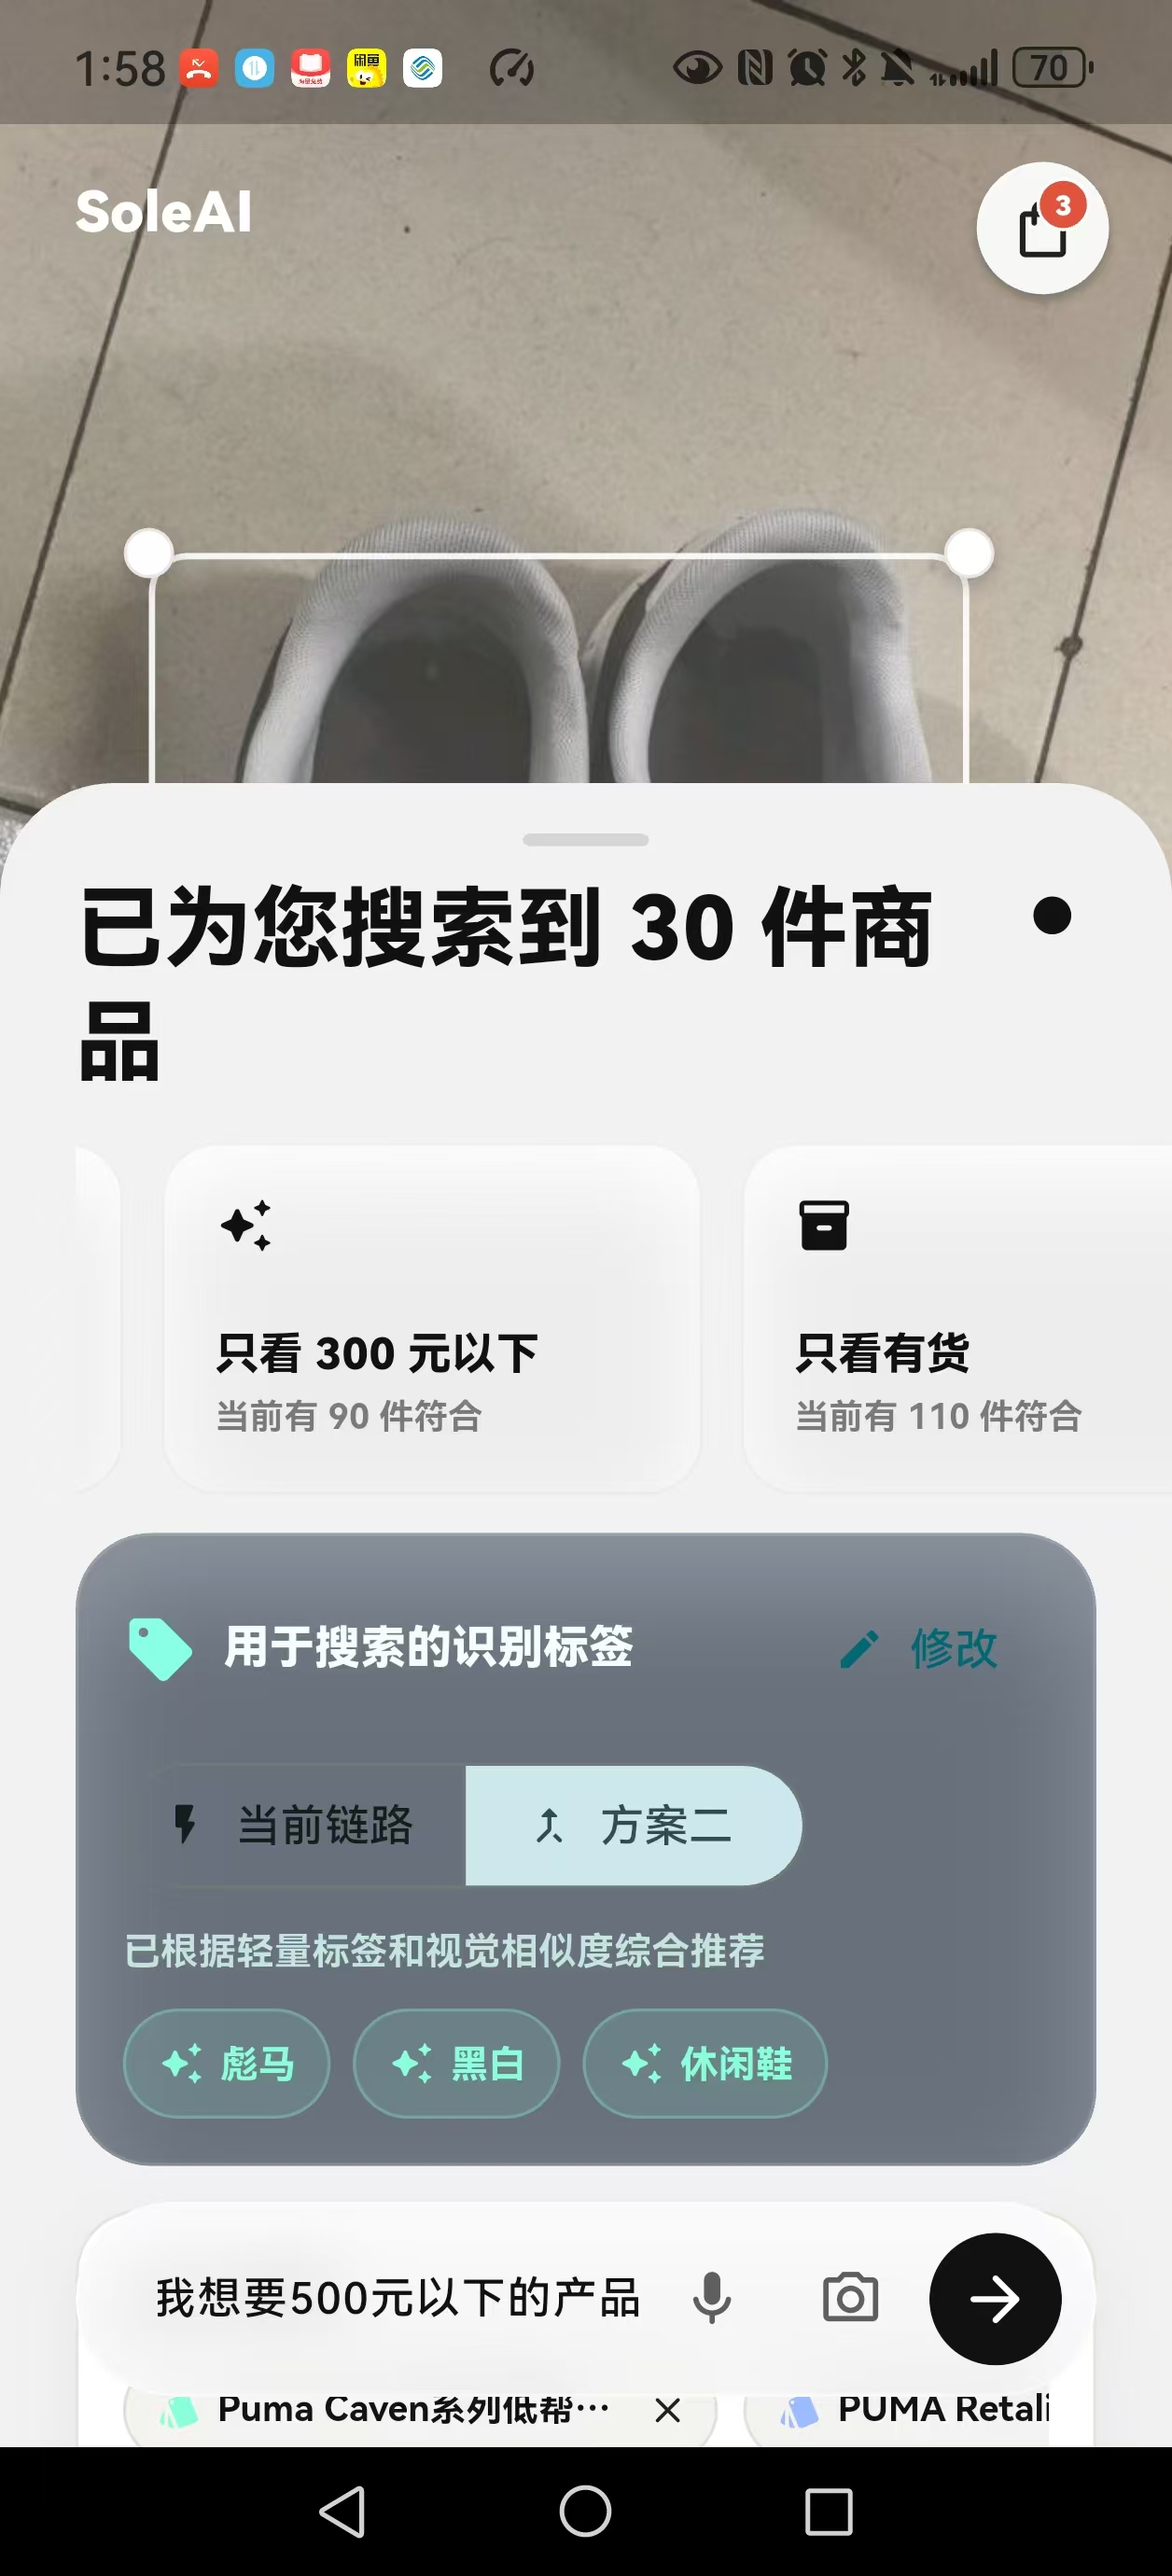
\includegraphics[width=\linewidth]{ui_result_profile.jpg}
  \caption{结果与画像}
\end{subfigure}
\hfill
\begin{subfigure}{0.23\textwidth}
  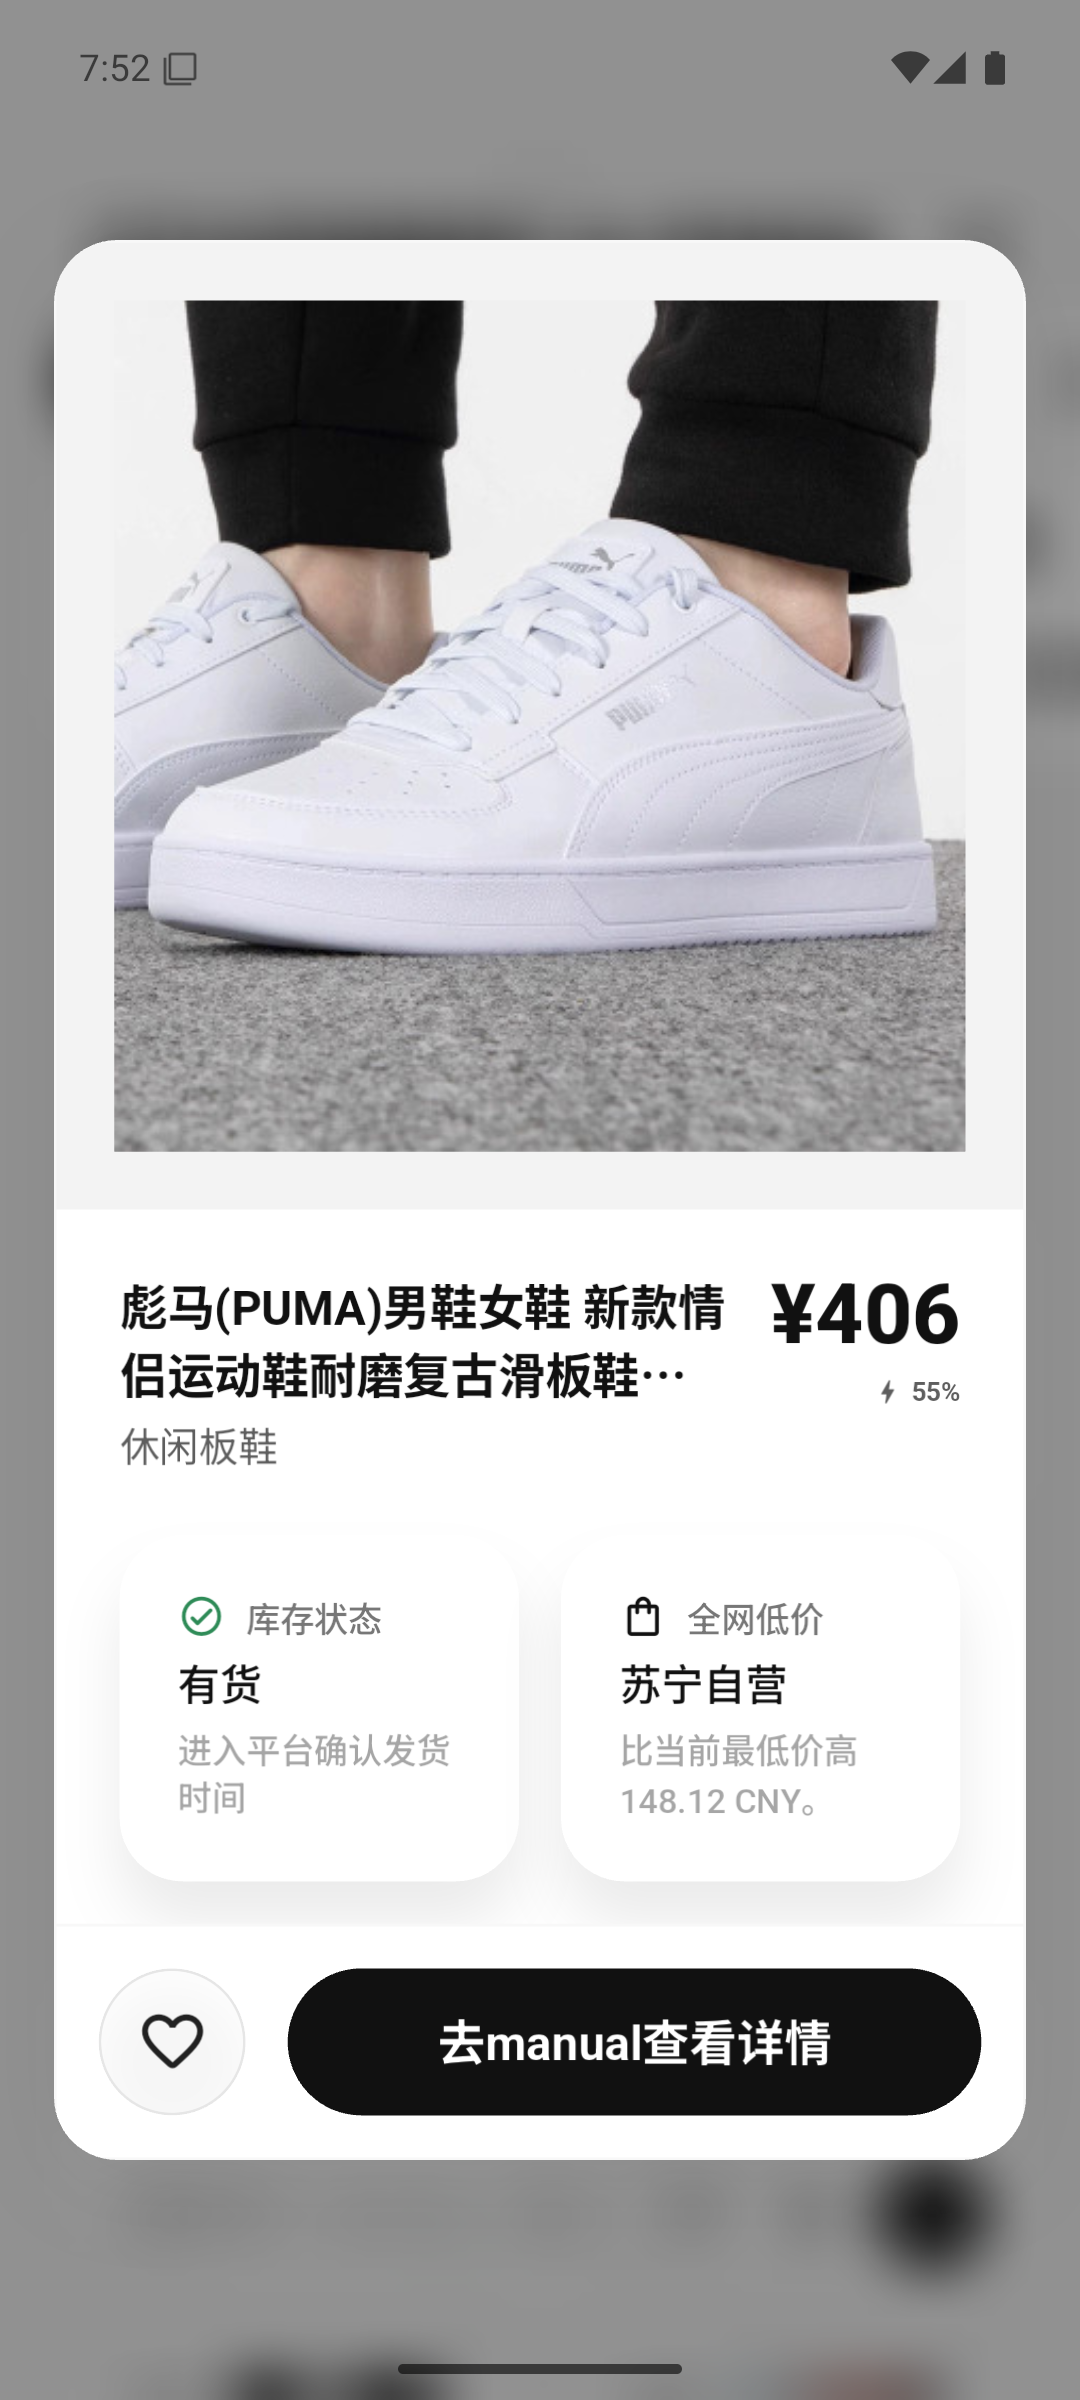
\includegraphics[width=\linewidth]{ui_detail_price.png}
  \caption{商品详情}
\end{subfigure}
\hfill
\begin{subfigure}{0.23\textwidth}
  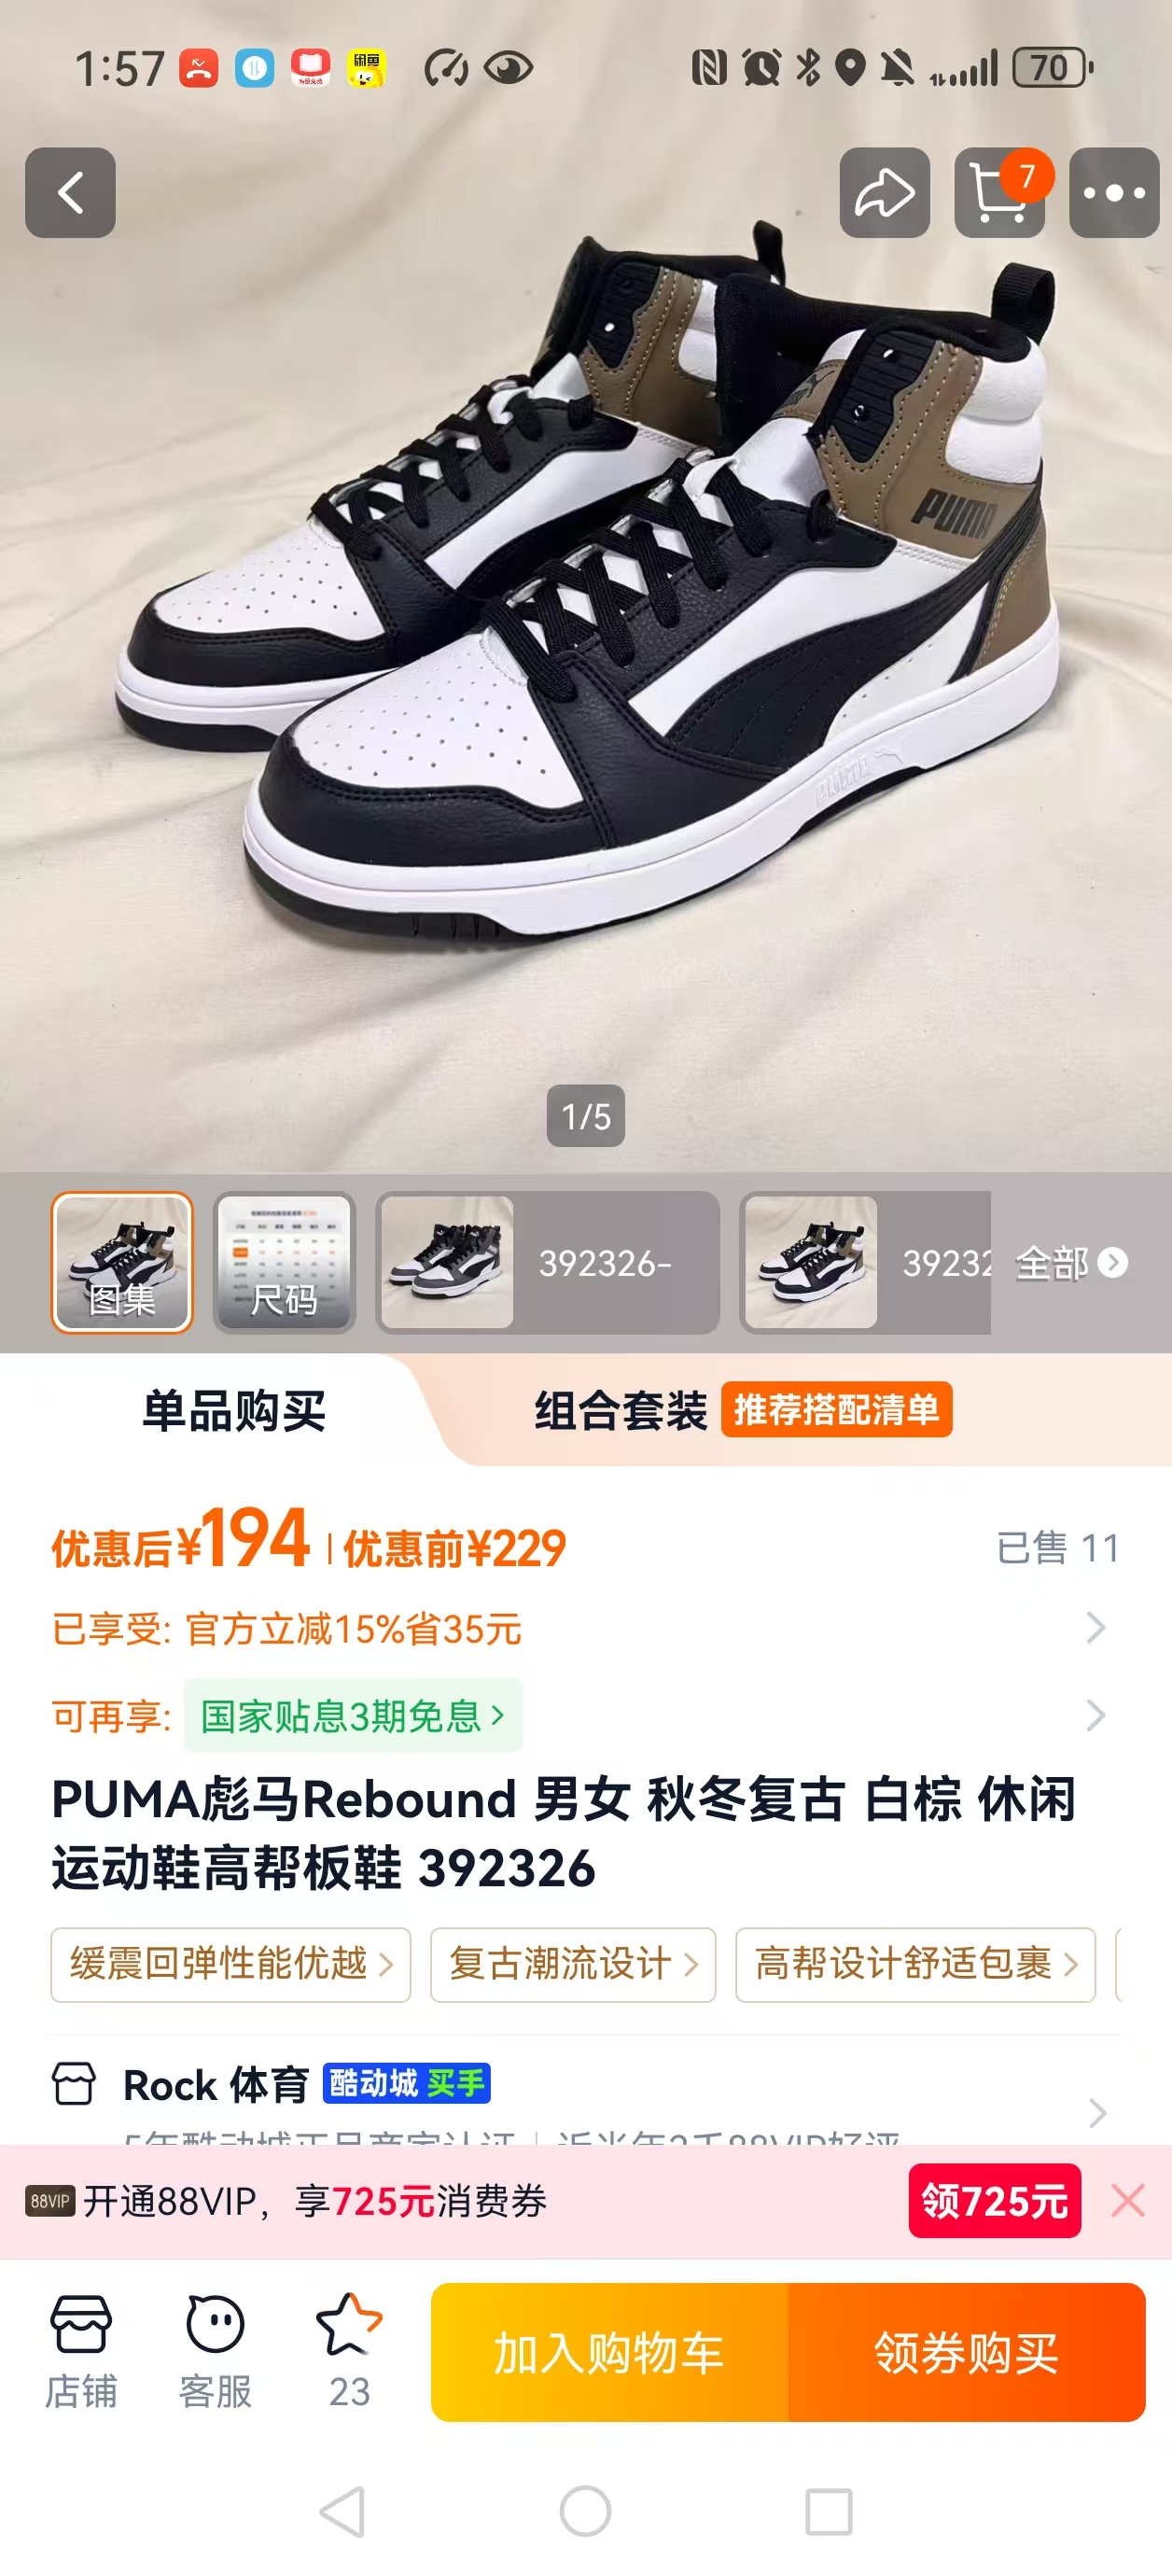
\includegraphics[width=\linewidth]{ui_external_product.jpg}
  \caption{购买落点}
\end{subfigure}
\caption{结果收敛、详情判断与购买落点}
\label{fig:refine-ui}
\end{figure}

\subsection{用户画像、购物车与推荐扩展}

除主搜索链路外，项目还实现了面向长期体验的用户画像编辑和会话购物车。用户画像用于减少重复输入，例如尺码、预算、偏好平台和排斥平台；会话购物车用于承接用户在当前搜索中关注的候选商品，并进一步触发 TrendOutfit 搭配推荐。

用户画像和购物车也是经过取舍后加入的。直接把所有偏好都自动记住，短期看起来智能，但容易保存错误或敏感信息；完全不记住用户，又会让用户每次都重复输入预算、尺码或平台偏好。因此后端采用 profile block 和 memory proposal：用户主动编辑的画像可以直接保存，系统从对话中抽取出的长期偏好需要用户确认后才写入。购物车则只保存当前会话中用户主动关注的候选，为后续搭配推荐提供明确上下文。

\begin{figure}[H]
\centering
\begin{subfigure}{0.23\textwidth}
  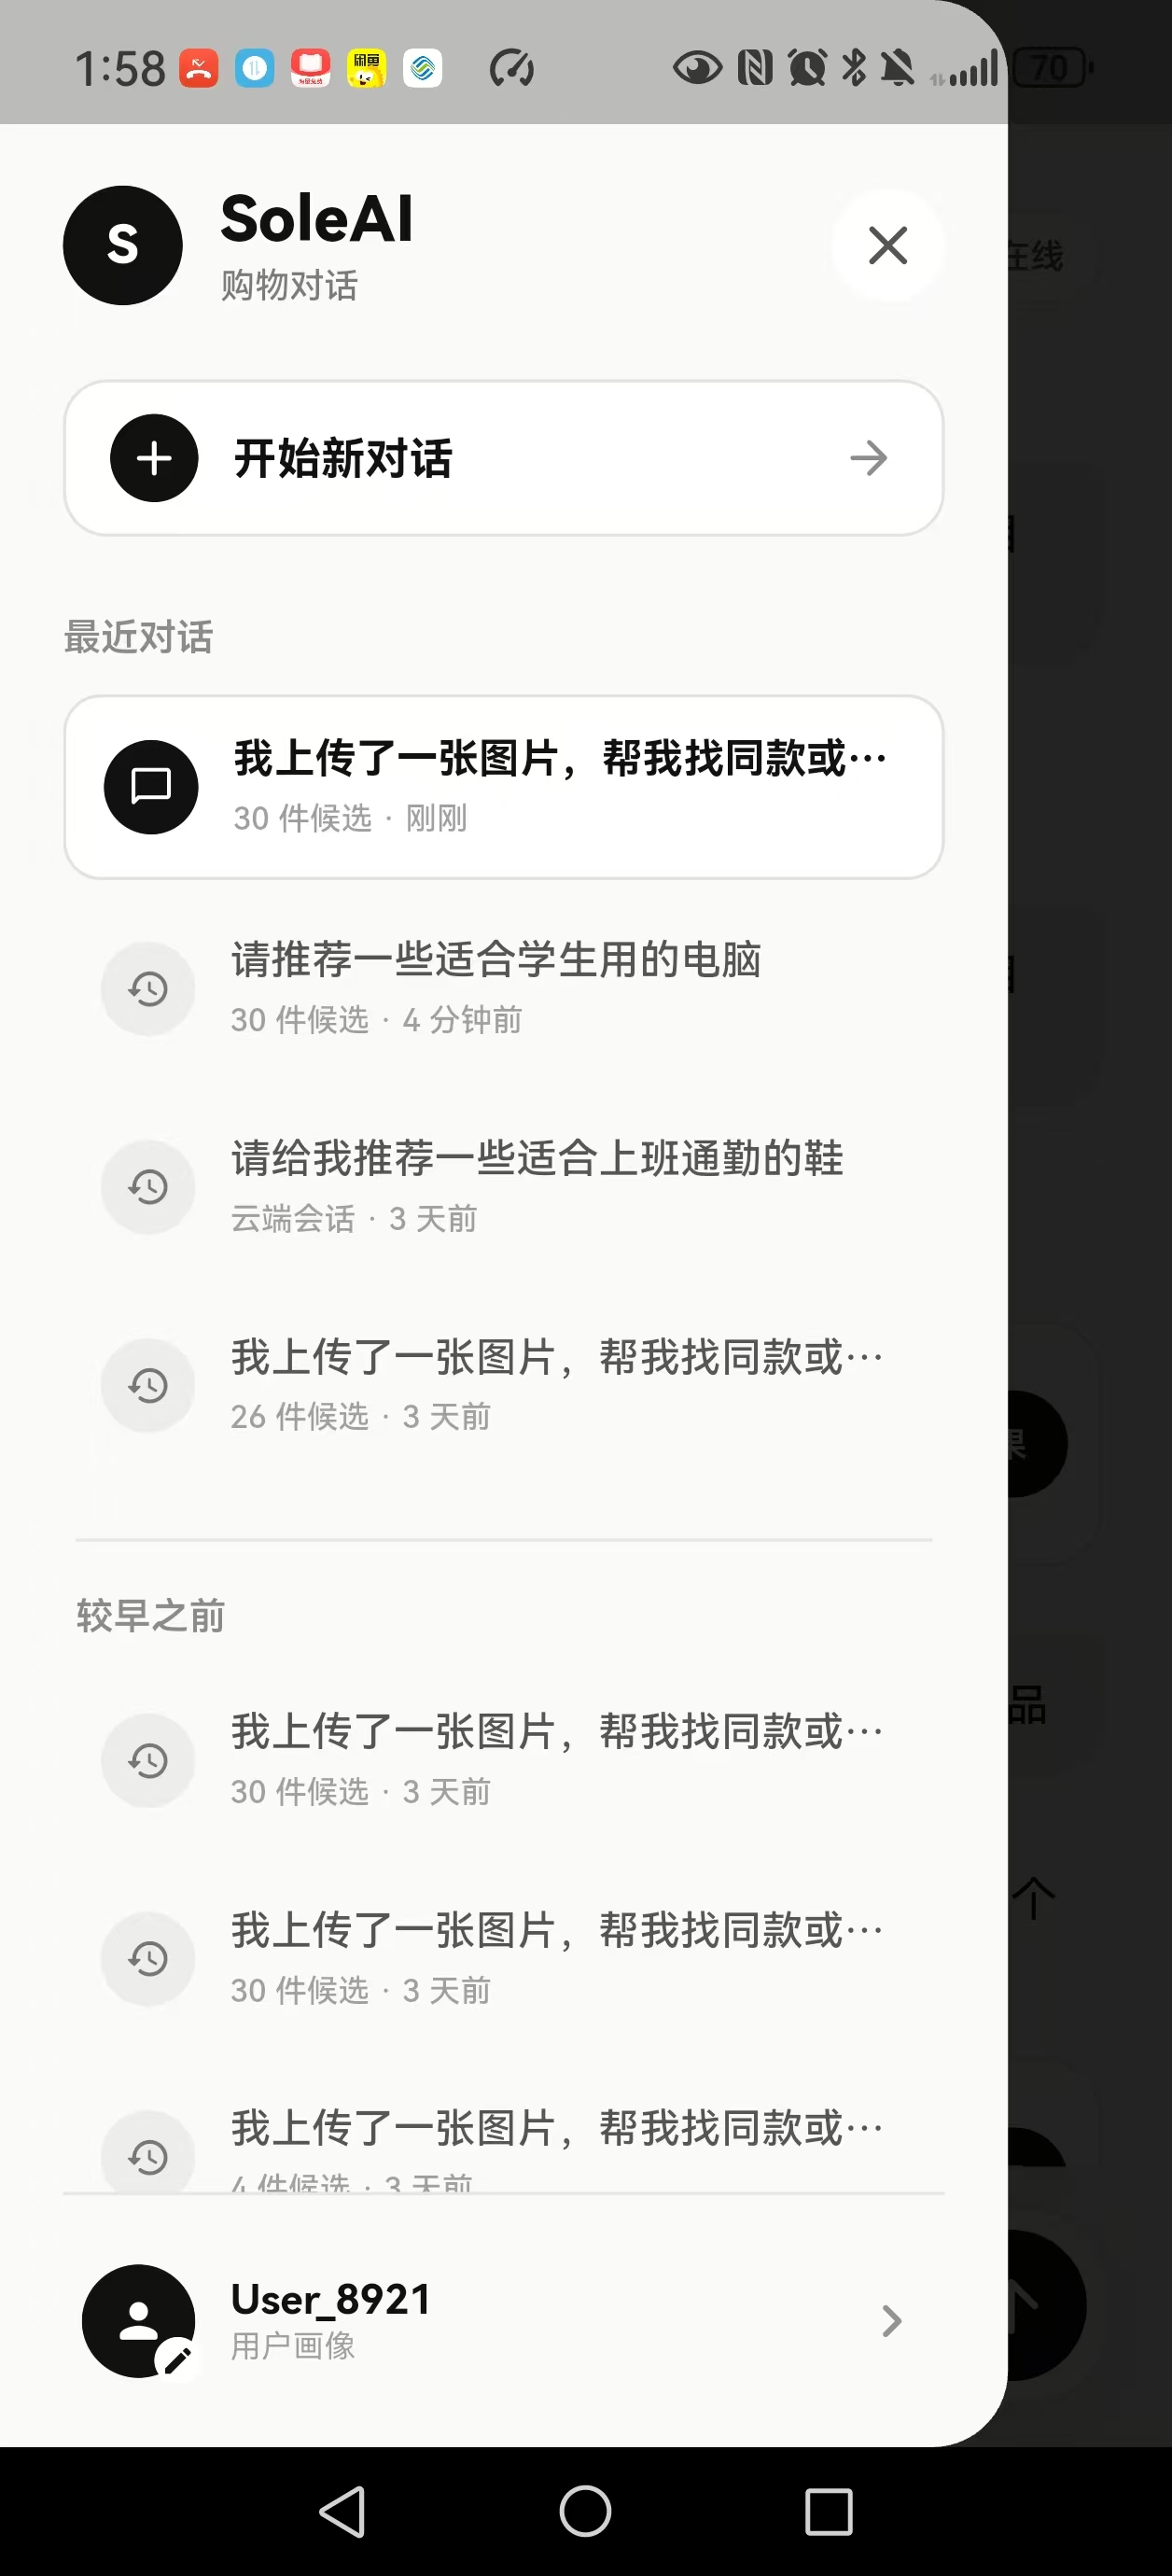
\includegraphics[width=\linewidth]{ui_drawer.jpg}
  \caption{会话侧栏}
\end{subfigure}
\hfill
\begin{subfigure}{0.23\textwidth}
  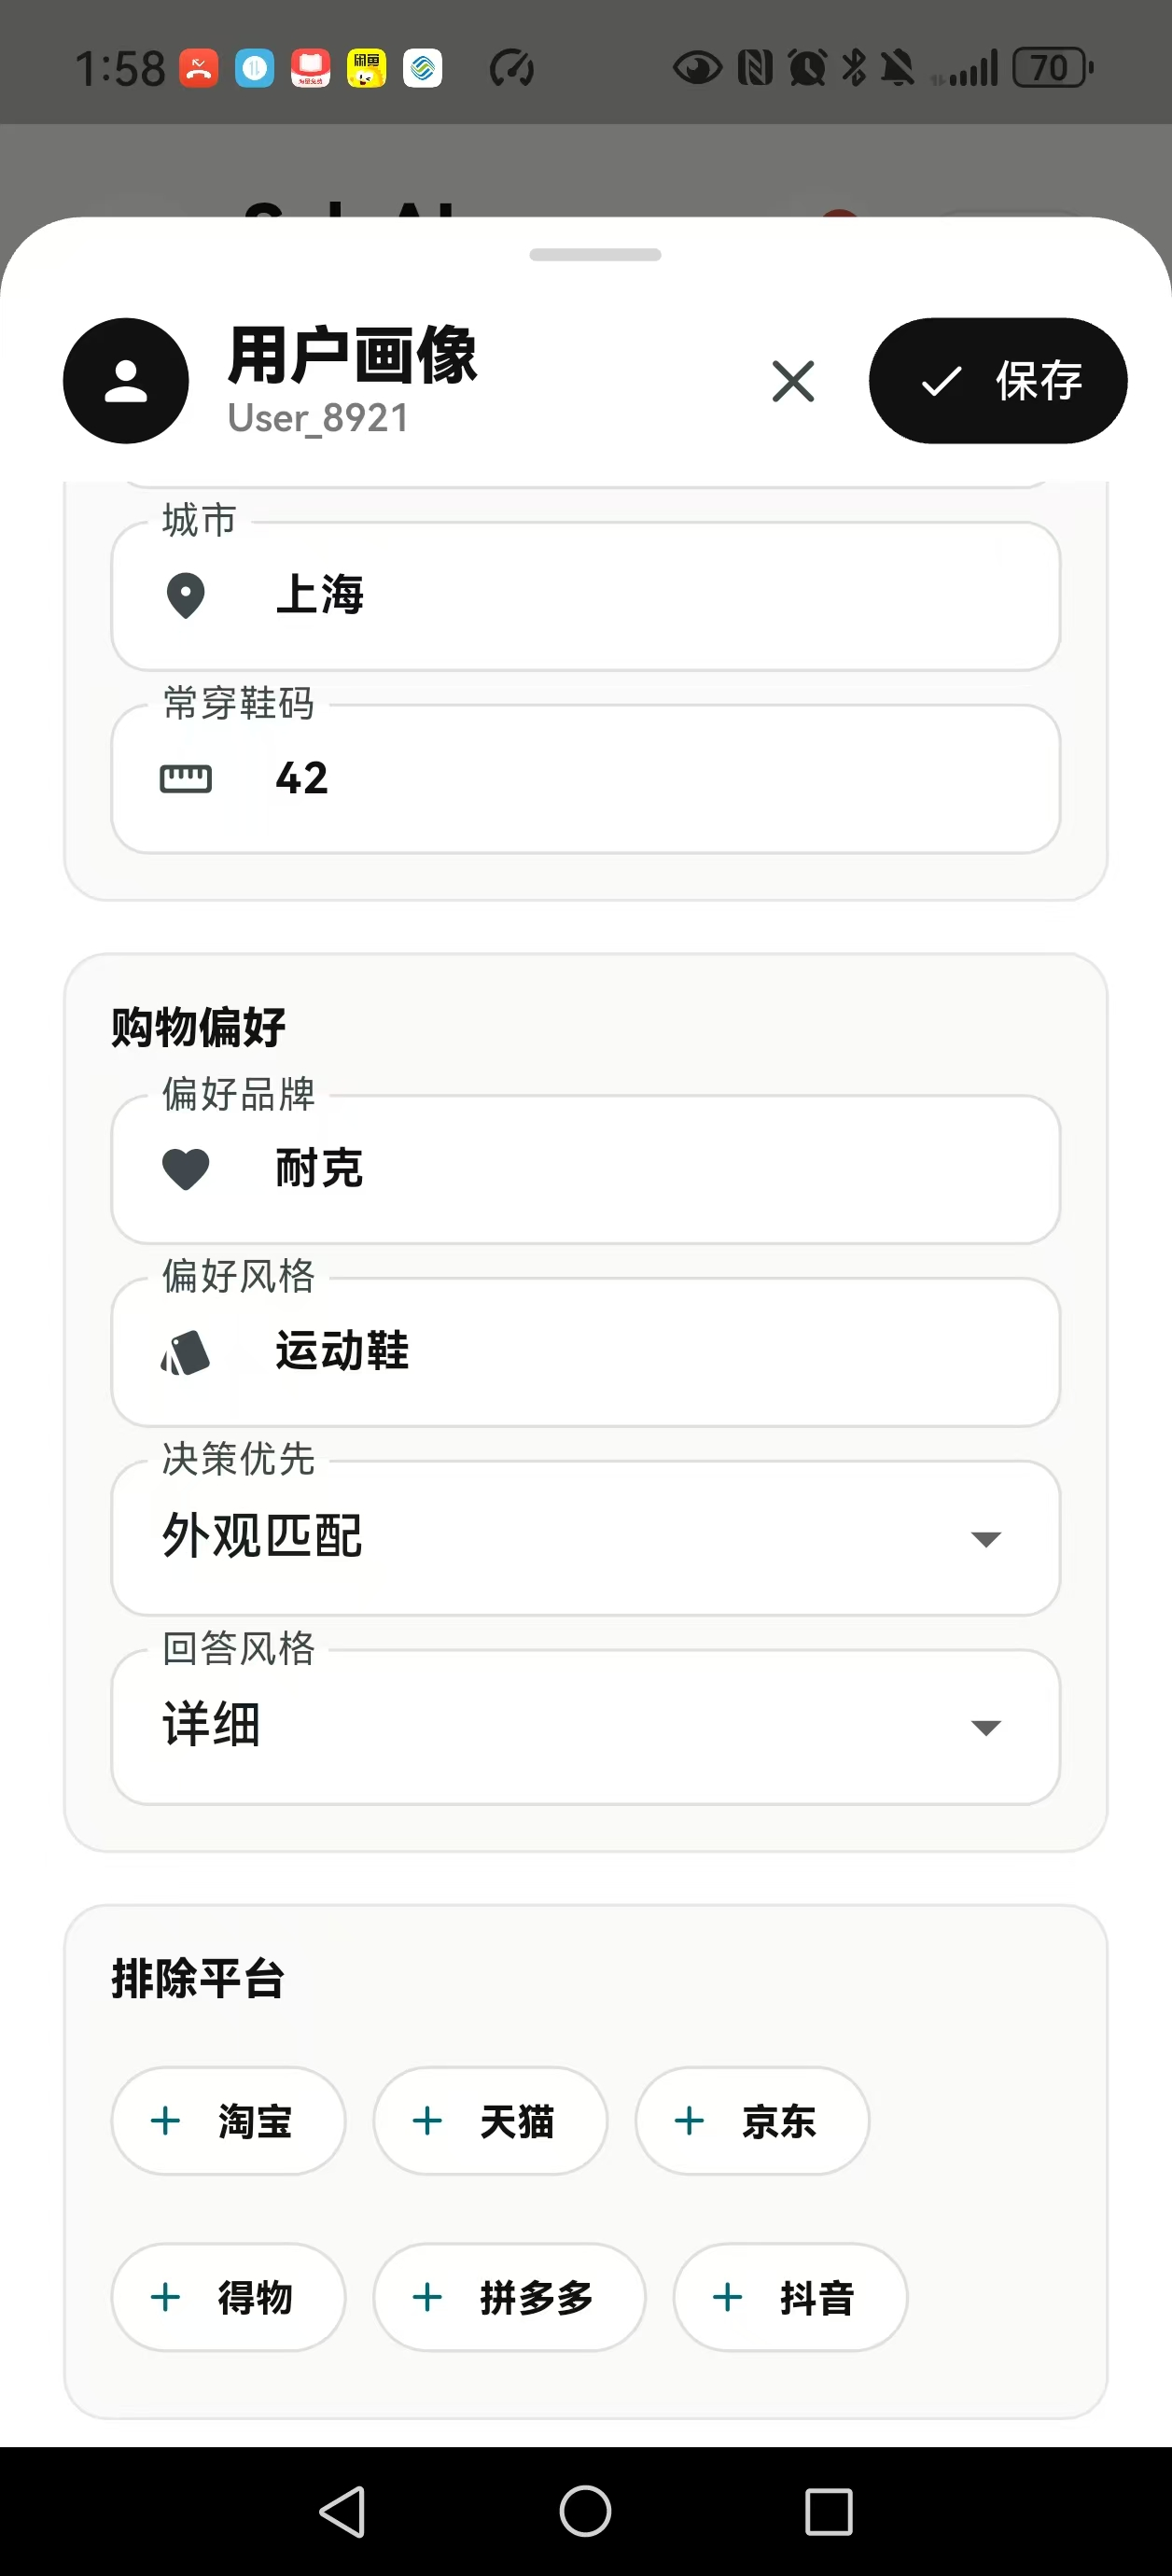
\includegraphics[width=\linewidth]{ui_profile_editor.jpg}
  \caption{用户画像编辑}
\end{subfigure}
\hfill
\begin{subfigure}{0.23\textwidth}
  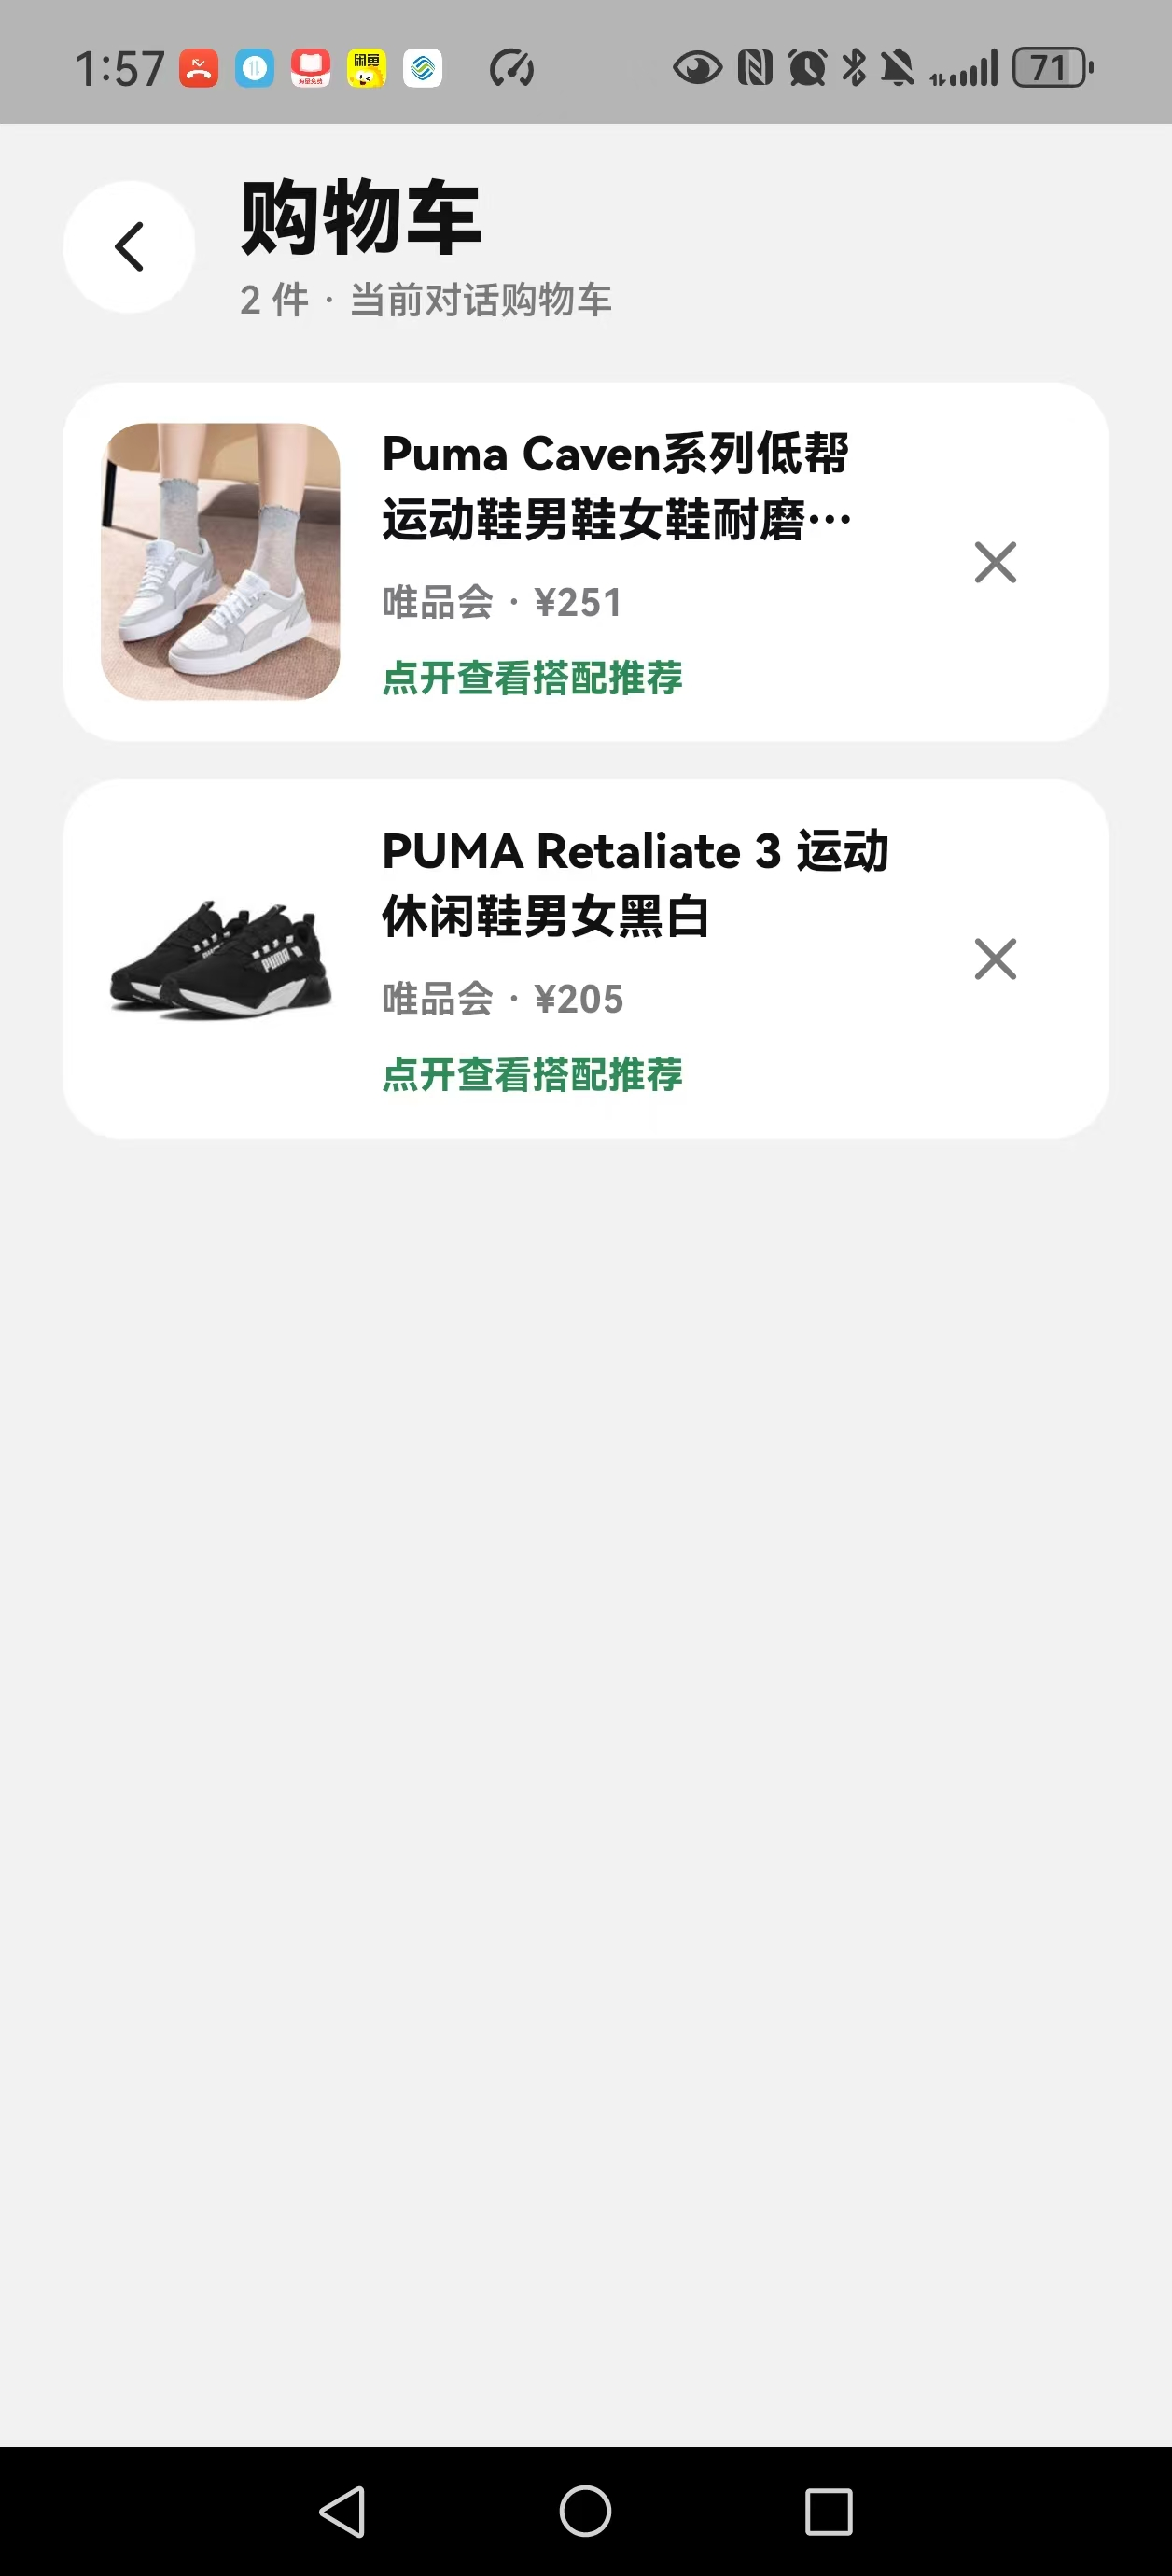
\includegraphics[width=\linewidth]{ui_cart.jpg}
  \caption{会话购物车}
\end{subfigure}
\hfill
\begin{subfigure}{0.23\textwidth}
  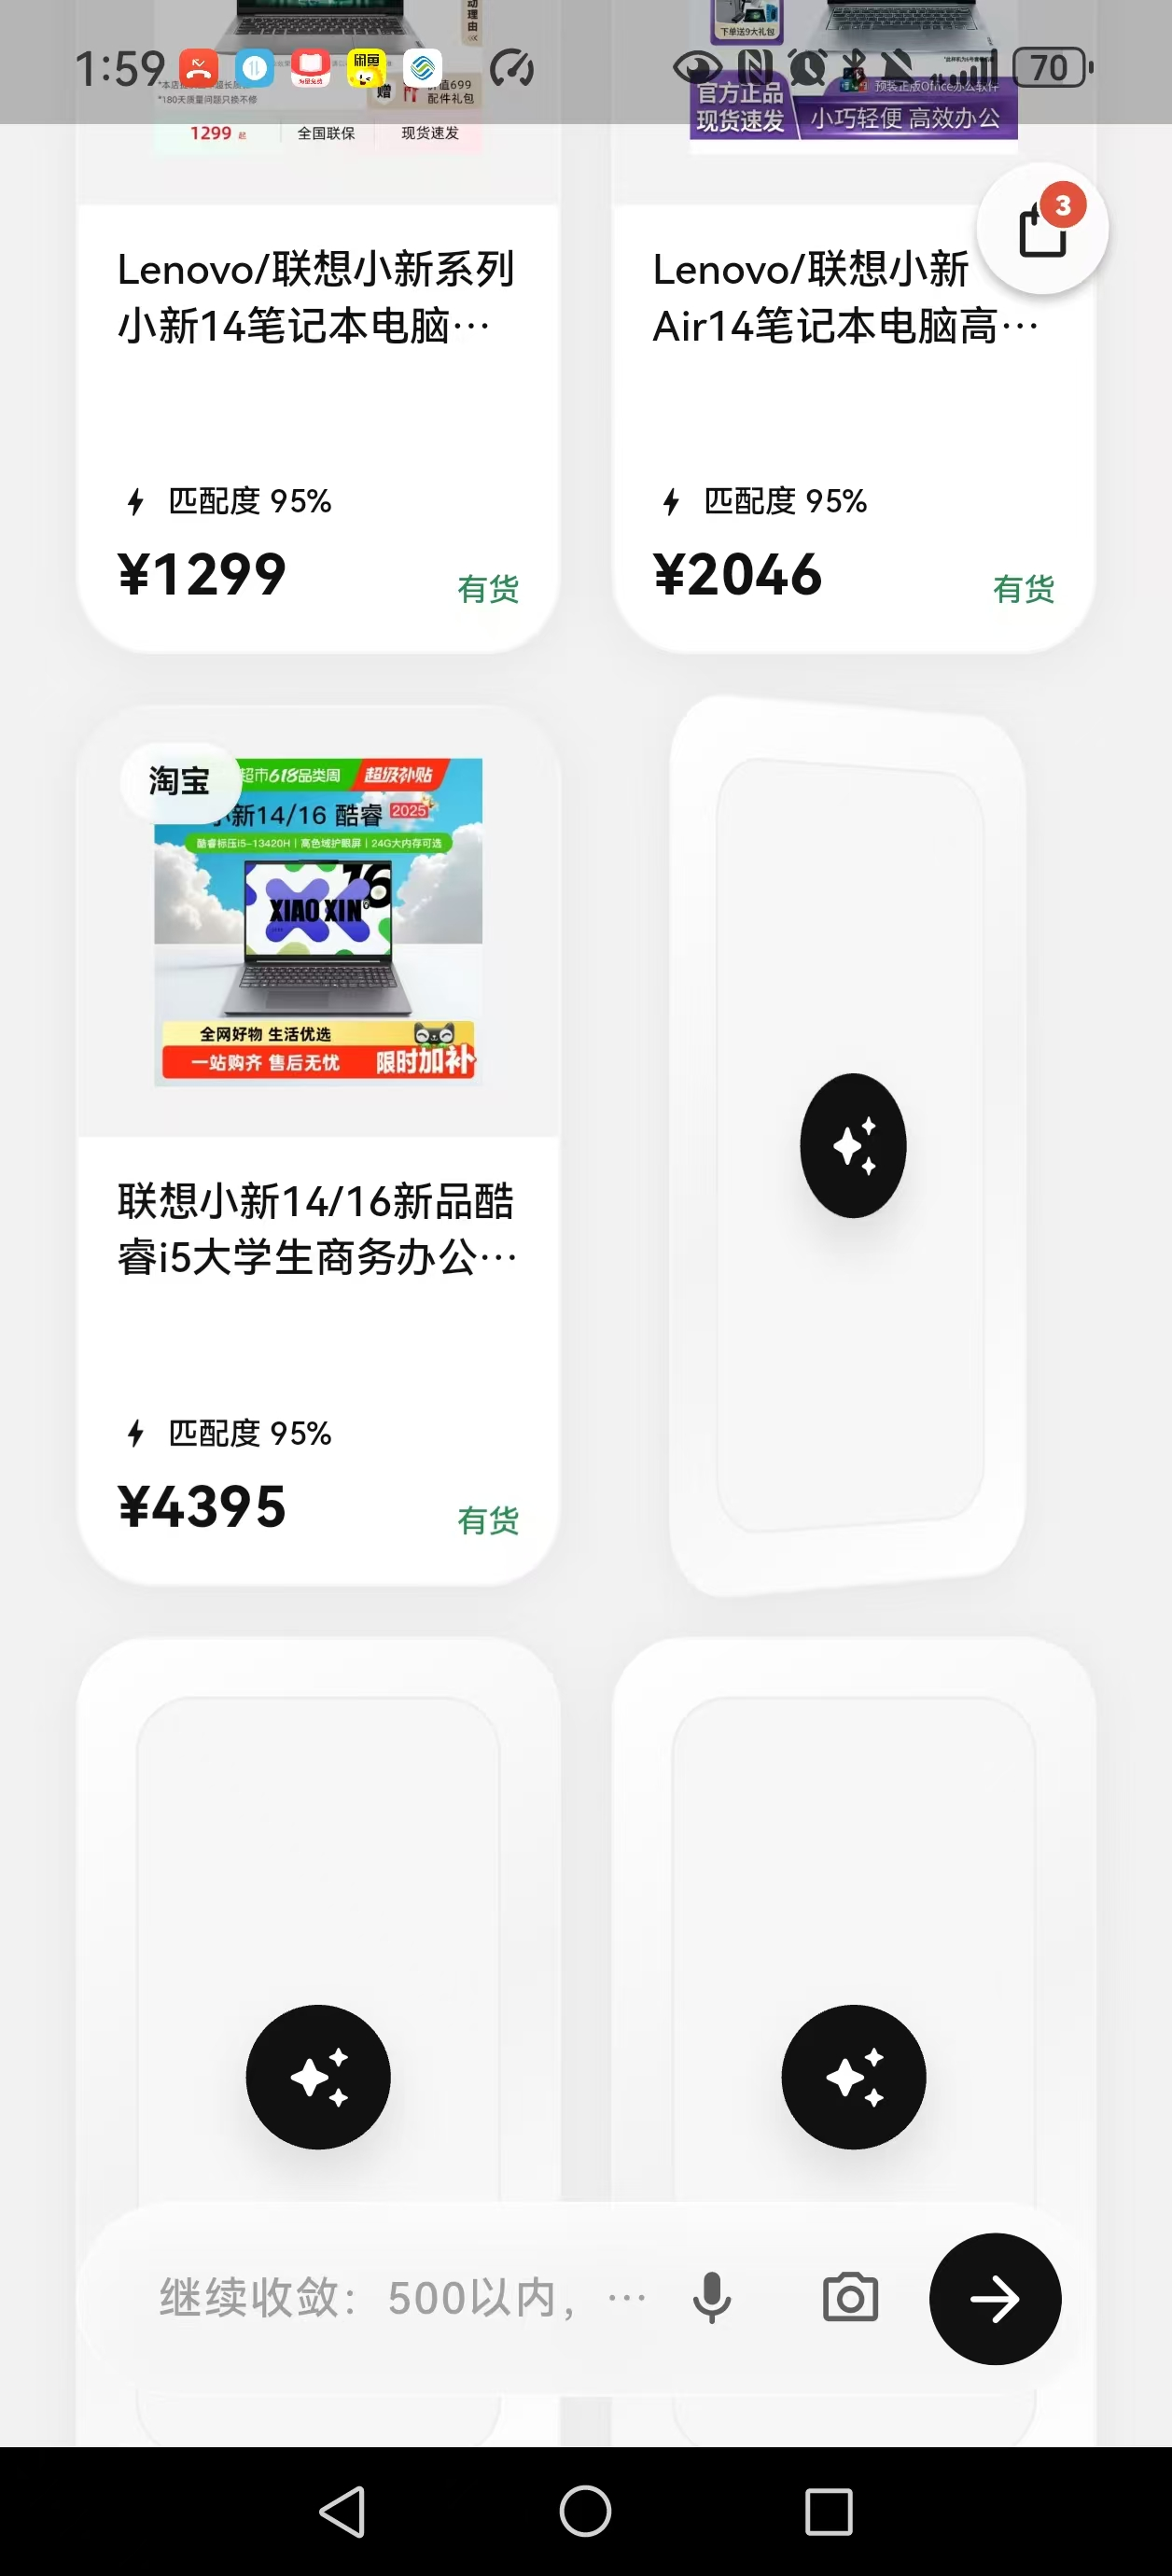
\includegraphics[width=\linewidth]{ui_general_results.jpg}
  \caption{扩展商品结果}
\end{subfigure}
\caption{长期偏好与推荐扩展界面}
\label{fig:profile-cart}
\end{figure}

\section{全品类搜索与候选生成链路}

\subsection{主链路概述}

项目当前主链路不是简单的“上传图片后调用一次模型”。我们实际做的是一条全品类商品搜索流水线：前端只负责采集图片和表达需求，后端负责把图片、标签、向量、商品池、筛选条件和候选快照串起来。鞋类截图只是演示样例，链路中的商品画像、商品池导入、平台字段标准化和候选展示都按通用商品对象设计。

\begin{center}
\code{上传图片 -> 主体定位 -> 商品画像 -> query embedding -> tag recall + ANN recall -> 融合排序 -> CandidateSnapshot}
\end{center}

图 \ref{fig:data-pipeline-main} 是我们整理的云端图片处理和结果生成数据通路。它展示了用户输入、图片资产、视觉模型、主体定位、向量检索、候选快照和前端输出之间的关系。把这张图放在正文中，是因为它正好解释了系统为什么不是一个“前端页面 + 大模型回答”的 demo，而是一条可观察、可恢复、可替换的数据处理链。

\begin{figure}[H]
\centering
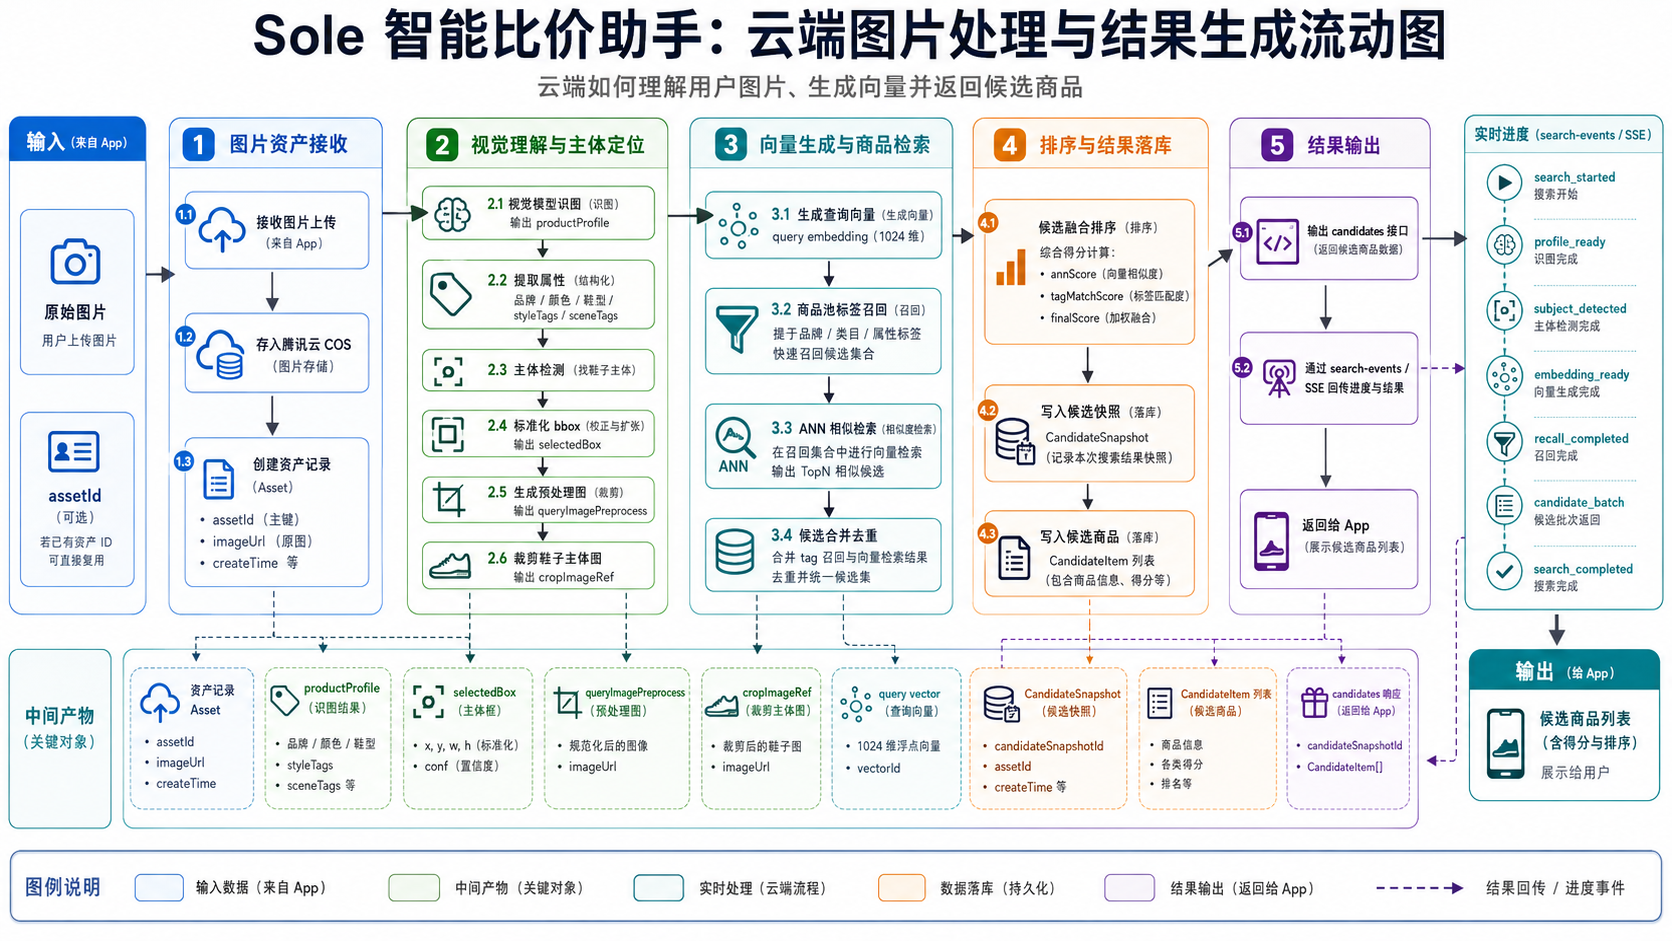
\includegraphics[width=0.95\textwidth]{pipeline_processing.png}
\caption{云端图片处理与结果生成数据通路}
\label{fig:data-pipeline-main}
\end{figure}

图 \ref{fig:image-pipeline} 把主链路进一步抽象成程序内部阶段。用户只看到图片上传和结果返回，后端内部则需要处理图片存储、主体框、标签、向量、候选池、分页和降级状态。

\begin{figure}[H]
\centering
\resizebox{\textwidth}{!}{
\begin{tikzpicture}[
  proc/.style={rectangle, rounded corners=2pt, draw=soleBlue, fill=lightBlue, minimum width=2.65cm, minimum height=0.82cm, align=center},
  data/.style={rectangle, rounded corners=2pt, draw=soleGreen, fill=lightGreen, minimum width=2.65cm, minimum height=0.82cm, align=center},
  warn/.style={rectangle, rounded corners=2pt, draw=soleOrange, fill=lightOrange, minimum width=2.65cm, minimum height=0.82cm, align=center},
  arrow/.style={-{Stealth[length=2.1mm]}, thick, draw=soleGray}
]
\node[proc] (upload) {图片上传\\Assets};
\node[proc, right=0.55cm of upload] (vision) {视觉识别\\productProfile};
\node[proc, right=0.55cm of vision] (crop) {主体裁剪\\normalized bbox};
\node[proc, right=0.55cm of crop] (embed) {生成 query\\embedding};
\node[data, below=0.75cm of vision] (tags) {品牌/颜色/品类\\标签召回};
\node[data, below=0.75cm of embed] (ann) {视觉向量\\ANN 召回};
\node[proc, right=0.55cm of embed] (merge) {去重融合\\综合排序};
\node[warn, right=0.55cm of merge] (snapshot) {候选快照\\分页与恢复};
\draw[arrow] (upload) -- (vision);
\draw[arrow] (vision) -- (crop);
\draw[arrow] (crop) -- (embed);
\draw[arrow] (vision) -- (tags);
\draw[arrow] (embed) -- (ann);
\draw[arrow] (tags.east) -| (merge.south);
\draw[arrow] (ann.east) -| (merge.south);
\draw[arrow] (embed) -- (merge);
\draw[arrow] (merge) -- (snapshot);
\end{tikzpicture}
}
\caption{全品类图片搜索与候选生成链路}
\label{fig:image-pipeline}
\end{figure}

\subsection{搜索链路的多次尝试与最终取舍}

后端搜索链路是本项目中最重要的工程取舍之一。我们不是一开始就得到当前方案，而是在等待时间、搜索精确度、解释性和用户可控性之间反复比较后，最终保留两种可切换模式，并默认采用 \code{light\_tag\_ann\_fusion}。

\begin{table}[H]
\centering
\caption{搜索链路尝试与取舍}
\label{tab:search-tradeoff}
\begin{tabularx}{\textwidth}{p{3.1cm}Y Y Y}
\toprule
方案 & 优点 & 问题 & 最终处理 \\
\midrule
纯文本或平台关键词搜索 & 实现简单，能快速返回一批结果 & 对图片输入不友好，依赖标题质量，无法利用视觉相似度 & 只作为商品数据源或后续补充，不作为主链路 \\
纯图片 ANN 召回 & 响应快，适合首屏返回视觉相似商品 & 用户难以理解结果来源，颜色/品牌/型号误差难以修正 & 保留为快速召回路径，但不单独承担最终推荐 \\
完整画像识别后再搜索 & 标签更完整，排序更容易解释 & 首屏等待时间长，视觉模型慢或失败时会阻塞搜索 & 作为对照模式 \apibreak{current\_ann\_then}{\_refine} 保留 \\
图片 + 标签混合 embedding & 看起来能统一图文语义 & 用户修改标签后，结果变化不够可解释；混合向量权重难以调试 & 暂不采用，避免把用户可控标签重新放进黑盒向量中 \\
轻量标签 + ANN 融合 & 首屏等待较短，同时保留标签解释和视觉召回 & 需要处理两路候选去重、阈值、排序和降级 & 作为默认展示模式 \apibreak{light\_tag\_ann}{\_fusion} \\
\bottomrule
\end{tabularx}
\end{table}

最终方案的关键点是：后端在一个短等待窗口内尽量生成轻量商品标签和 profile；如果轻量标签生成失败或超时，系统仍可退化到纯图 ANN，不让识别失败中断整条搜索链路。标签召回提供可解释约束，ANN 召回提供视觉相似兜底，融合排序负责把两路结果合成用户看到的候选列表。对于不同品类，前端只展示适合该品类的核心标签，例如品牌、主色、品类、型号或款式；鞋类演示中这些标签表现为品牌、颜色、鞋型。

\begin{figure}[H]
\centering
\resizebox{0.95\textwidth}{!}{
\begin{tikzpicture}[
  box/.style={rectangle, rounded corners=2pt, draw=soleGray, fill=lightGray, minimum width=3.2cm, minimum height=0.82cm, align=center},
  blue/.style={rectangle, rounded corners=2pt, draw=soleBlue, fill=lightBlue, minimum width=3.2cm, minimum height=0.82cm, align=center},
  green/.style={rectangle, rounded corners=2pt, draw=soleGreen, fill=lightGreen, minimum width=3.2cm, minimum height=0.82cm, align=center},
  purple/.style={rectangle, rounded corners=2pt, draw=solePurple, fill=lightPurple, minimum width=3.2cm, minimum height=0.82cm, align=center},
  arrow/.style={-{Stealth[length=2.2mm]}, thick, draw=soleGray}
]
\node[box] (profile) {用户图像\\商品画像};
\node[blue, right=1.0cm of profile, yshift=0.8cm] (tag) {Route A\\品牌/品类标签召回};
\node[green, right=1.0cm of profile, yshift=-0.8cm] (ann) {Route B\\视觉 ANN 召回};
\node[purple, right=1.2cm of tag, yshift=-0.8cm] (merge) {融合去重\\阈值过滤与排序};
\node[box, right=1.2cm of merge] (topk) {Top K 候选\\统一 CandidateItem};
\draw[arrow] (profile) -- (tag);
\draw[arrow] (profile) -- (ann);
\draw[arrow] (tag) -- (merge);
\draw[arrow] (ann) -- (merge);
\draw[arrow] (merge) -- (topk);
\end{tikzpicture}
}
\caption{ProductPool 中标签召回与 ANN 召回的融合}
\label{fig:fusion}
\end{figure}

\subsection{商品池与多平台数据通路}

为了让应用支持全品类和多平台，我们没有把某一次爬取结果写死在搜索逻辑中，而是先把外部数据清洗为统一商品契约，再进入 ProductPool。不同平台的字段可能叫“标题”“商品名称”“goodsName”，价格可能是字符串、区间或促销价，图片可能是单图或多图。ProductPool 的作用是把这些差异转成统一的 Product、ProductImageEmbedding、CandidateItem 和 rawPayload。

图 \ref{fig:data-pool-flow} 展示商品数据从外部平台进入系统后的处理方式。这里的重点不是“有没有某个平台 API”，而是系统已经具备了商品导入、字段标准化、批次审计、图片标准化、embedding 生成和候选返回的完整通路。

\begin{figure}[H]
\centering
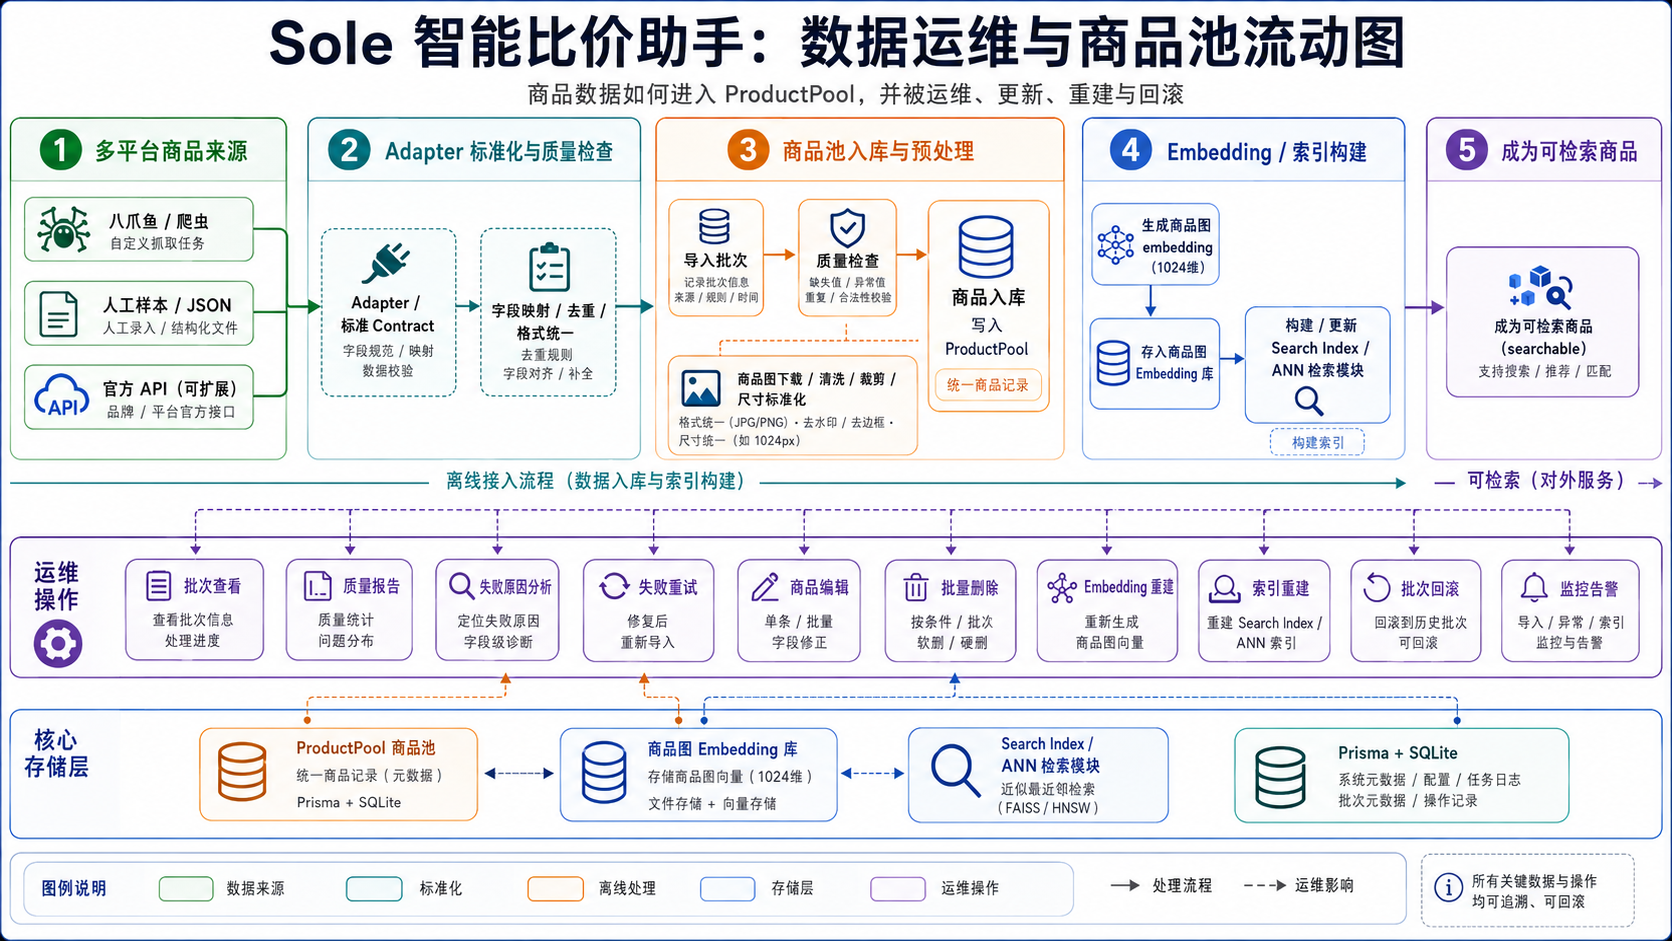
\includegraphics[width=0.95\textwidth]{data_pool_flow.png}
\caption{多平台商品数据进入 ProductPool 的数据通路}
\label{fig:data-pool-flow}
\end{figure}

图 \ref{fig:upload-result-flow} 展示从用户上传到结果返回的完整路径。该图对应前端体验中的“拍照/上传 - 等待搜索 - 查看候选”三个阶段，也解释了为什么我们需要 CandidateSnapshot：当用户继续筛选或点击查看更多时，系统优先复用当前会话的候选快照，而不是每次都重新调用模型和搜索。

\begin{figure}[H]
\centering
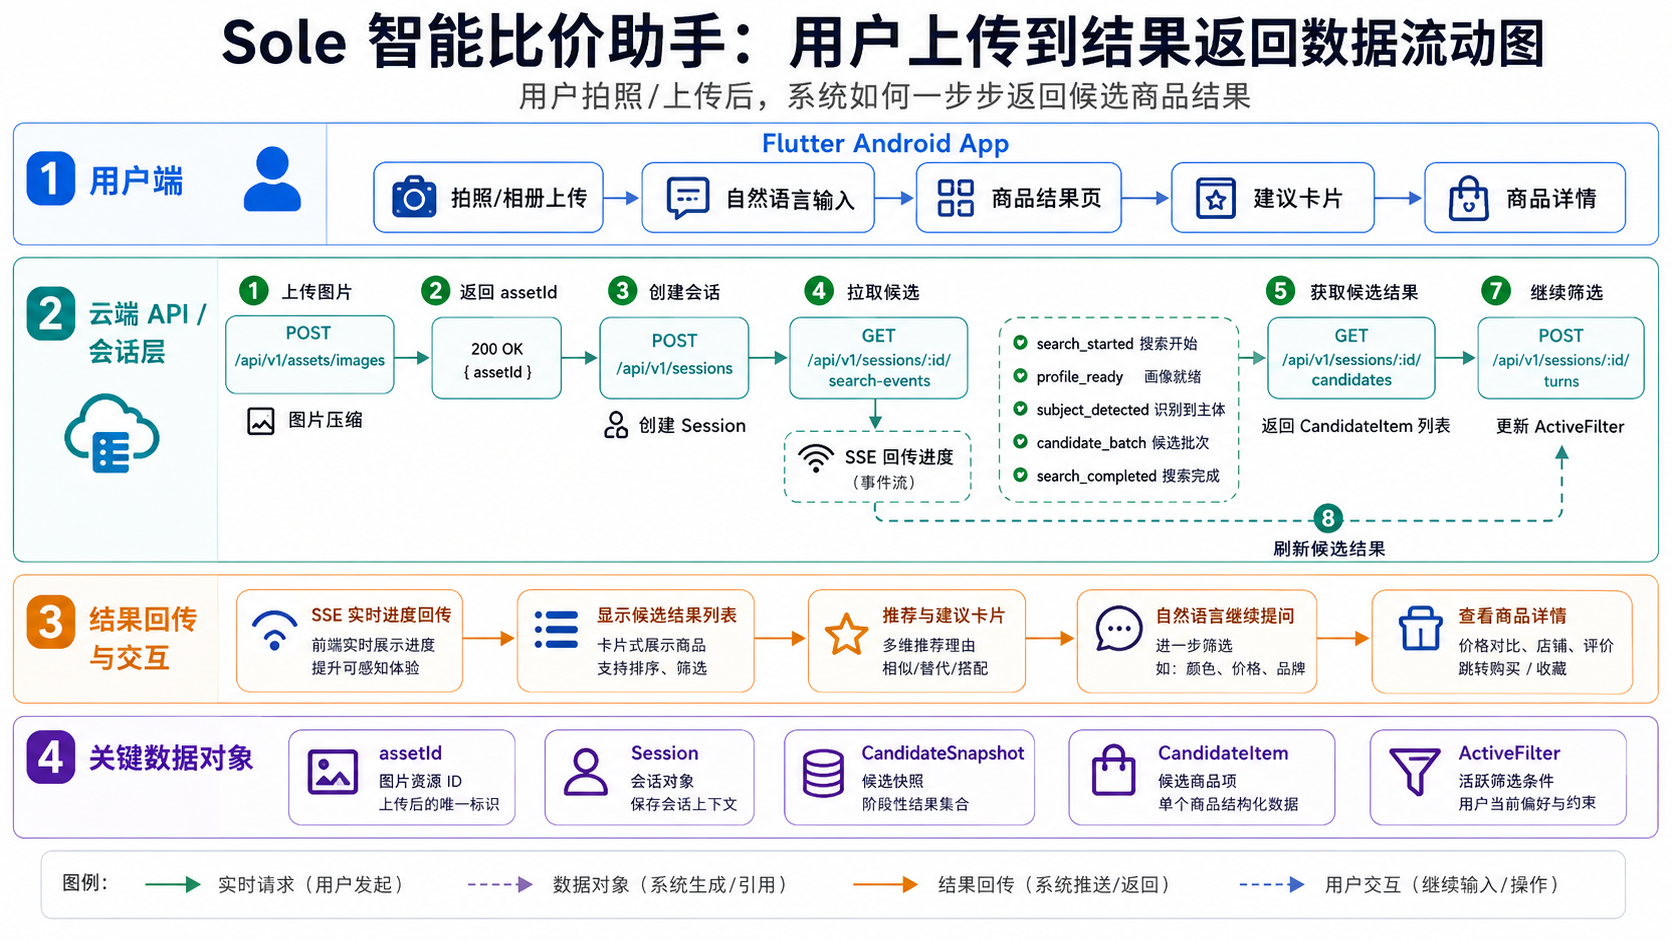
\includegraphics[width=0.95\textwidth]{upload_to_results_flow.png}
\caption{用户上传图片到候选结果返回的数据通路}
\label{fig:upload-result-flow}
\end{figure}

\subsection{多轮筛选与候选快照}

多轮筛选的关键不是“重新发起一次搜索”，而是在同一会话中合并筛选条件并利用当前候选快照刷新结果。图 \ref{fig:sequence} 展示一个典型时序。

\begin{figure}[H]
\centering
\resizebox{\textwidth}{!}{
\begin{tikzpicture}[
  actor/.style={rectangle, rounded corners=2pt, draw=black!45, fill=lightGray, minimum width=2.2cm, minimum height=0.7cm, align=center},
  msg/.style={-{Stealth[length=2mm]}, draw=soleGray, thick},
  lifeline/.style={draw=black!25, dashed}
]
\node[actor] (user) {用户};
\node[actor, right=2.2cm of user] (app) {Flutter App};
\node[actor, right=2.2cm of app] (api) {NestJS API};
\node[actor, right=2.2cm of api] (pool) {ProductPool};
\node[actor, right=2.2cm of pool] (model) {LLM/VLM};
\foreach \x in {user,app,api,pool,model} \draw[lifeline] (\x.south) -- ++(0,-5.8);
\draw[msg] ($(user.south)+(0,-0.5)$) -- node[above, font=\small] {输入“500 元以内”} ($(app.south)+(0,-0.5)$);
\draw[msg] ($(app.south)+(0,-1.2)$) -- node[above, font=\small] {POST /turns} ($(api.south)+(0,-1.2)$);
\draw[msg] ($(api.south)+(0,-1.9)$) -- node[above, font=\small] {解析 filterPatch} ($(model.south)+(0,-1.9)$);
\draw[msg] ($(api.south)+(0,-2.6)$) -- node[above, font=\small] {读取快照与候选池} ($(pool.south)+(0,-2.6)$);
\draw[msg] ($(pool.south)+(0,-3.3)$) -- node[above, font=\small] {过滤/重排结果} ($(api.south)+(0,-3.3)$);
\draw[msg] ($(api.south)+(0,-4.0)$) -- node[above, font=\small] {候选 + 建议} ($(app.south)+(0,-4.0)$);
\draw[msg] ($(app.south)+(0,-4.7)$) -- node[above, font=\small] {刷新列表} ($(user.south)+(0,-4.7)$);
\end{tikzpicture}
}
\caption{自然语言追加筛选的会话时序}
\label{fig:sequence}
\end{figure}

这一设计也是一个取舍。完全无状态接口实现简单，但用户每一句追加要求都会变成新的搜索，体验上像“重新来过”；完全依赖前端状态又会导致 App 退出、网络中断或后端重启后结果丢失。因此我们把当前商品画像、筛选条件和候选列表写入候选快照（\mbox{\code{CandidateSnapshot}}），由数据库承担可恢复状态，进程内缓存只做加速层。这样用户继续输入“只看有货”“500 元以内”“不要某个平台”时，系统可以在当前候选池上继续收敛，也可以在候选不足时补充检索。

\subsection{我们完成的能力落点}

本项目完成的内容可以按“用户可见能力”和“后端支撑能力”两类理解。用户可见能力包括：拍照/相册上传、主体框选、核心标签展示与编辑、候选结果列表、自然语言多轮筛选、建议卡片、商品详情、会话购物车、用户画像编辑和搭配推荐。后端支撑能力包括：图片对象存储、模型 Adapter、商品池导入、图片 embedding、ANN 检索、标签召回、候选快照、分页游标、用户记忆、缓存和云端 smoke 验证。

这些能力不是孤立按钮，而是围绕一个目标组织：让用户用更少操作完成“找到商品 - 比较结果 - 继续筛选 - 判断是否购买”的完整过程。例如可编辑标签解决 AI 识别错误带来的不可控问题；候选快照解决多轮筛选时反复等待的问题；TrendOutfit 保持独立接口，是为了扩展搭配场景但不干扰基础搜索稳定性；用户画像采用 block 和待确认 proposal，是为了让长期偏好参与筛选，同时避免系统自动记住错误或敏感信息。

\subsection{其他关键实现取舍}

除了搜索链路本身，项目中还有多处类似的权衡。表 \ref{tab:engineering-tradeoffs} 总结了几个最重要的决策。它们共同体现了项目的工程目标：不是堆功能，而是在可演示、可维护、可解释和可扩展之间找到当前课程项目最合适的实现方式。

\begin{table}[H]
\centering
\caption{关键实现取舍}
\label{tab:engineering-tradeoffs}
\begin{tabularx}{\textwidth}{p{3cm}Y Y}
\toprule
问题 & 可选方案与风险 & 最终实现 \\
\midrule
商品数据来源 & 直接实时调聚合搜索 API 上手快，但外部波动大，字段不可控；只用 mock 数据稳定但没有真实度。 & 建立 ProductPool，把多平台、多品类数据先标准化、审计、生成 embedding，再供搜索链路使用；聚合 API 保留为可替换 provider。 \\
图片存储 & 图片二进制直接进数据库会让 SQLite 膨胀，文件系统路径又不适合云端部署。 & 图片进入对象存储，数据库只保存 objectKey、URL、尺寸、变体类型和会话关系。 \\
识别结果呈现 & 把模型识别结果藏在后端最省界面，但用户无法纠错；全部字段暴露又会增加认知负担。 & 前端只展示真正参与搜索的核心标签，如品牌、主色、品类/型号，并允许用户修改后重新检索。 \\
多轮筛选状态 & 完全无状态接口简单，但每轮像重新搜索；完全靠前端状态则难恢复。 & 后端保存会话、筛选条件和 CandidateSnapshot；前端负责输入与展示，后端负责连续性。 \\
搭配推荐 & 把 TrendOutfit 混入主搜索链路能少写接口，但会影响基础图片搜索稳定性。 & 单独实现推荐模块和接口，从购物车或候选商品触发，主搜索链路保持独立。 \\
缓存策略 & 直接上 Redis 更完整但部署复杂；完全不用缓存会增加重复识别和搜索等待。 & MVP 使用 NestJS 进程内轻缓存加 SQLite 快照，缓存只加速，不作为正式状态来源。 \\
\bottomrule
\end{tabularx}
\end{table}

\section{优点与不足}

\subsection{主要优点}

\begin{table}[H]
\centering
\caption{项目优势分析}
\begin{tabularx}{\textwidth}{p{3.1cm}Y Y}
\toprule
维度 & 优点 & 具体体现 \\
\midrule
交互体验 & 输入方式自然，用户门槛低 & 图片上传和自然语言追问构成核心交互，不要求用户学习复杂筛选器。 \\
结果可控 & 用户可以纠正识别标签 & 前端展示品牌、颜色、品类、型号等核心标签，避免 AI 识别错误完全隐藏在后台。 \\
工程架构 & 外部能力可替换 & 模型、Embedding、商品源、对象存储、ANN 都通过 Adapter 或 Port 隔离。 \\
会话连续性 & 支持多轮上下文 & 候选快照、筛选状态和 turns 使用户不用每次重新搜索。 \\
数据资产 & 商品池可审计、可回滚 & ProductPool 支持批次导入、质量报告、embedding 覆盖和运维入口。 \\
展示完整度 & 移动端流程接近真实产品 & 首页、主体选择、结果列表、详情、画像编辑、购物车等界面较完整。 \\
\bottomrule
\end{tabularx}
\end{table}

\subsection{当前不足}

\begin{table}[H]
\centering
\caption{当前不足与影响}
\begin{tabularx}{\textwidth}{p{3.1cm}Y Y}
\toprule
维度 & 不足 & 影响 \\
\midrule
商品数据规模 & 真实商品池仍偏小 & 召回覆盖范围有限，无法证明对大量品牌和平台都稳定。 \\
价格真实性 & 历史价格链路仍为基础展示或预留 & 不能完整回答“现在是否值得买”的长期价格问题。 \\
配送时效 & 预计送达时间未接入真实来源 & 目前主要按价格和匹配度辅助判断，时效维度不足。 \\
用户研究 & 缺少正式可用性测试数据 & HCI 效果主要来自设计推理和功能验证，缺少任务时间、错误率、满意度量化。 \\
跨平台体验 & 主体验集中在 Android APK & iOS 或纯 Web 用户无法完整体验原生拍照链路。 \\
隐私解释 & 用户画像和上传图片的说明还可加强 & 长期偏好、图片存储、删除机制需要更清楚地展示给用户。 \\
\bottomrule
\end{tabularx}
\end{table}

\section{改进方向}

\subsection{数据与检索改进}

后续应扩大真实商品池规模，覆盖更多品类、品牌、价格段和平台，并为每次导入保留质量报告。检索侧可以继续优化标签召回和 ANN 召回的权重，增加人工标注的正负样本，用 Precision@K、Recall@K 和首屏相关性评估来衡量改进。

\subsection{HCI 评估改进}

建议设计小规模用户研究，让参与者完成固定任务，例如“用一张商品图找到 500 元以内的同款或近似款”“排除某个平台后找到有货候选”“修改识别标签后重新检索”。记录完成时间、追问次数、误点次数、结果满意度和主观负担评分。这样可以把“省事”从设计目标转化为可量化证据。

\subsection{可访问性与错误恢复}

当前界面以视觉体验为主，后续应加入更清晰的错误反馈、加载阶段说明、无障碍标签、字号适配和对低网速场景的恢复提示。对于模型失败、上传失败、候选为空等状态，应明确告诉用户“发生了什么、还能做什么”。

\subsection{交付体验改进}

课程交付可以继续采用 APK + Web 入口，但建议补充免安装 Web 体验页。Web 体验页只需支持图片上传、创建会话、候选展示和文本筛选，即可成为评委无法安装 APK 时的备用路径。

\subsection{隐私与长期画像改进}

用户画像功能已经具备基础接口和编辑入口。后续应在产品层加入更明确的说明：哪些信息会被记住、为什么记住、如何删除、是否会影响搜索结果。长期记忆必须保持用户确认后生效，避免系统自动写入敏感或错误偏好。

\section{结论}

SoleAI 当前已经从单纯界面演示推进到包含移动端、后端、商品池、AI 编排、检索融合、多轮筛选和推荐扩展的完整课程项目形态。它的核心贡献不只是调用视觉模型识别商品，而是把图片理解、商品数据、候选检索、自然语言筛选和决策辅助整合为一条用户可感知的交互链路。

从 HCI 角度看，项目把用户的操作负担从“多平台重复搜索和筛选”转移为“上传图片并用自然语言继续表达需求”。从工程角度看，项目通过 Adapter-first 架构、ProductPool、候选快照和可插拔检索链路，为后续扩展更多品类、更多平台和更多前端入口保留了空间。当前主要不足在于真实数据规模、正式用户研究、历史价格与配送时效仍需继续加强。整体而言，SoleAI 已经具备作为 HCI 期末大项目提交的完整说明基础和可演示系统基础。

\appendix

\section{团队贡献表}

团队成员信息尚未提供。最终提交前应将表 \ref{tab:team} 中的占位符替换为真实姓名、学号和贡献比例。

\begin{table}[H]
\centering
\caption{团队成员贡献占位表}
\label{tab:team}
\begin{tabularx}{\textwidth}{p{3cm}p{3cm}p{5cm}p{2.2cm}}
\toprule
姓名 & 学号 & 主要贡献 & 比例 \\
\midrule
待补充 & 待补充 & Flutter 客户端、交互流程、截图整理 & 待补充 \\
待补充 & 待补充 & NestJS 后端、商品池、检索链路、部署 & 待补充 \\
待补充 & 待补充 & HCI 分析、文档、测试与演示材料 & 待补充 \\
待补充 & 待补充 & 数据整理、评估、补充功能或答辩 & 待补充 \\
\bottomrule
\end{tabularx}
\end{table}

\section{最终提交检查清单}

\begin{itemize}
  \item 报告 PDF 是否能打开，且中文字体正常。
  \item 运行 README 是否包含后端、Web、Flutter 和 smoke 命令。
  \item 成员姓名、学号和贡献表是否已补齐。
  \item APK 或演示入口是否与 README 中的地址一致。
  \item 报告中的截图是否清晰、无缺失、无错误路径。
  \item 是否明确说明了系统能力、优点、不足和改进方向。
\end{itemize}

\end{document}
